%!TEX root = ../dissertation.tex
%\begin{savequote}[60mm]
%There is no scientific study more vital to man than the study of his own brain. Our entire view of the universe depends on it.\qauthor{Francis Crick}
%\end{savequote}

\begin{savequote}[70mm]
One of the difficulties in understanding the brain is that it is like nothing so much as a lump of porridge.\qauthor{Richard L. Gregory}
\end{savequote}

\chapter[microRNA Dynamics in Cholinergic Differentiation\texorpdfstring{\\}{} of Human Neuronal Cells]{microRNA Dynamics in Cholinergic Differentiation of Human Neuronal Cells}
This chapter will discuss the current state of knowledge on brain transcriptomics, generally and in the specific case of cholinergic neurons in the \ac{cns}, and then go on to explain the steps we undertook to elucidate small RNA processes in central cholinergic systems. First, our aim was to clarify co-expression patterns of central cholinergic neurons, which required analysis of transcriptome data in single-cell resolution. Based on this information, we selected two human models of cholinergic neuronal differentiation and established a differentiation protocol amenable to RNA extraction and successive molecular biology assays, most importantly, \ac{seq}. The expression patterns so obtained were then used to perform bioinformatics analyses using the database introduced in Chapter \ref{sec:database:mirnet}, \textit{miRNeo}. 

%!TEX root = ../dissertation.tex
\section{Neuronal Transcriptomes - Background}
The mammalian brain requires a constant supply of oxygen and nutrients, because it does not provide storage for either. Though it only makes up approximately 2\% of the entire human body mass, its energy expenditure is around 20\% of the whole.\cite{Raichle2002} For this reason, each square millimetre of brain tissue (except for the ventricles) is infiltrated by hundreds of capillaries.\cite{Bohn2016} Since the blood-brain-barrier is essentially provided by supporting glia cells surrounding all capillaries from the »inside« (see Fig.\,\ref{fig:bbb}, modified from Lobentanzer \& Klein\cite{Lobentanzer2019b}), neurons numerically constitute only a minority of brain tissues (but burn two thirds of its energy).

\begin{figure}
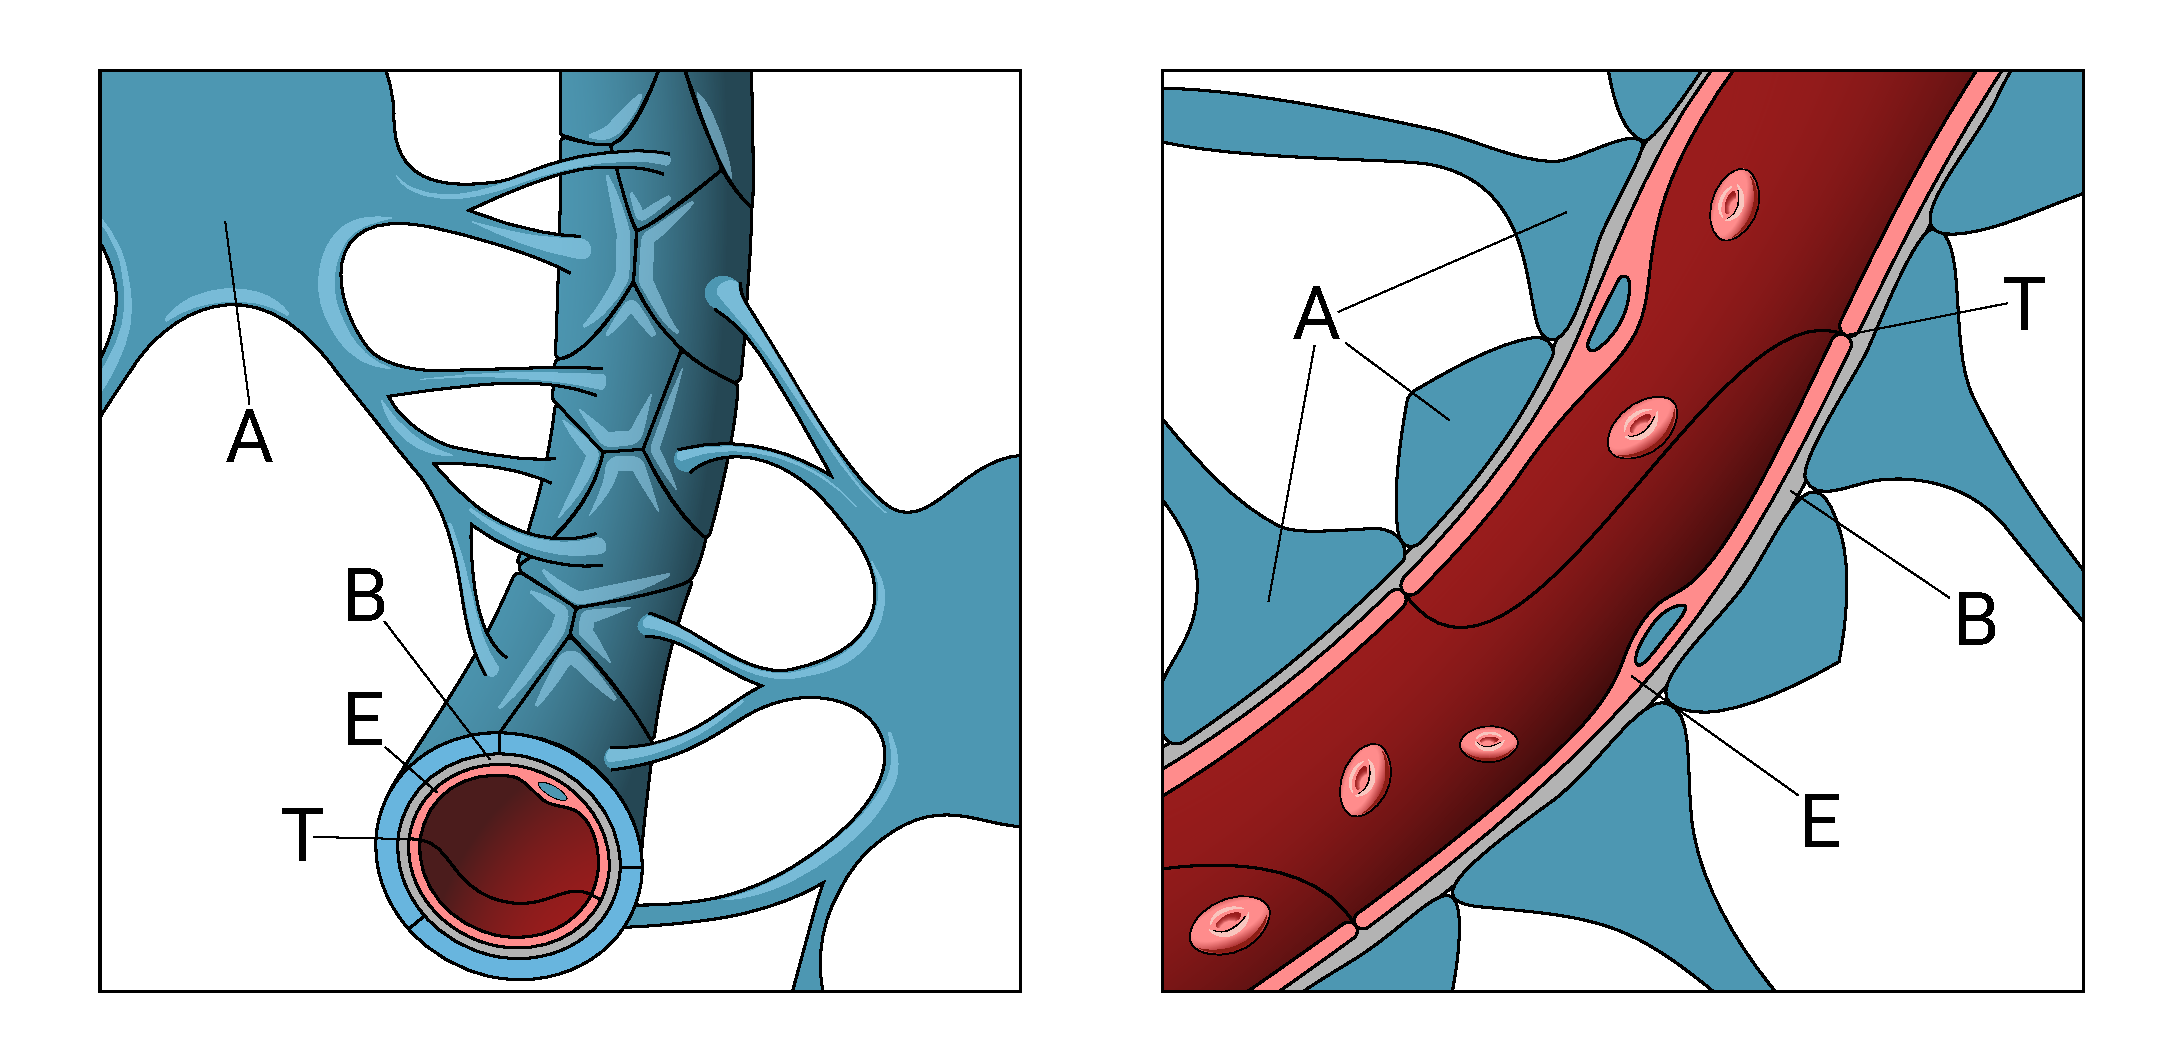
\includegraphics[width=\textwidth]{figures/bbb}
\caption[The blood-brain-barrier.]{\textbf{Schematic display of the blood-brain-barrier.} The blood-brain-barrier surrounds virtually every capillary in the CNS. A: Astrocyte, B: Basal Membrane, E: Endothelial Cell, T: Tight Junction. Modified from Lobentanzer \& Klein, 2019.\cite{Lobentanzer2019b}
\label{fig:bbb}}
\end{figure}

Until very recently, studies aiming to clarify the transcriptional profiles of neurons applied either microarray technology or \ac{seq} (also known as deep sequencing or next generation sequencing). For these methods, several cubic millimetres of brain tissue are required at the least; often, cubic centimetres are used. In contrast, the diameter of neuronal somata is usually in the micrometre range. Thus, the resolution of the method and the actual cellular resolution differ by a factor of approximately \num{1000}. Additionally, even among the neuronal population, there is considerable heterogeneity and transcriptomic plurality; single brain regions rarely consist of less than 30 different neuron types, tightly packed next to each other, each with their own transcriptional identity.\cite{Darmanis2015, Zeisel2015, Tasic2016, Habib2016} Newest studies, deciphering the murine nervous system by sequencing of \num{500000} individual cells, show that neuron diversity is very similar regardless of brain region.\cite{Zeisel2018} These circumstances hold true for any mammal, and most of our knowledge stems from the analysis of our favourite research animal, the mouse. In humans, the diversity is only exacerbated; in fact, the elevation in \ac{cns} complexity, which is only made possible by enhanced transcriptional control, may be the reason for our superior cognitive abilities(cite).

Cholinergic neurons always constitute a minority in any neuronal population, sometimes to extremes. Most tissues are dominated by few neuron types, such as pyramidal cells in the cortex. The most common neurotransmitter types are GABAergic (inhibitory) and glutamatergic (excitatory), each with several subtypes. It is estimated that more than 80\% of cortical neurons are excitatory, and more than 90\% of synapses release glutamate.\cite{Raichle2002} There are two major cholinergic regions in the mammalian brain: The striatum is fairly well-populated with rather large cholinergic interneurons, and the basal forebrain holds a large amount of (smaller) cholinergic projection neurons (compare Fig.\,\ref{fig:projections}). However, in transcriptomic analyses, these tissues are seldom used, maybe due to lack of scientific interest, or because they are notoriously hard to access (the basal forebrain is small and deeply imbedded in the midbrain). The cortex, particularly the neocortex, is most often the tissue of choice in these studies, due to its scientific interest and accessibility. Though it contains only a miniscule amount of cholinergic interneurons whose transcriptional identity is still a matter of debate, several of the recent single-cell \ac{seq} approaches have independently identified cholinergic interneurons in cortical regions (see Fig.\,\ref{fig:singlecell}).

\section{Cortical Single-Cell RNA Sequencing} \label{sec:cellculture:singlecell}
\newthought{The impact of transcriptional dynamics} on any disease depends on co-expression of the relevant genes in the affected cell. Selection of a model therefore has to take co-expression into account. In particular, if neurokines are to possess any relevance for cholinergic properties of central nervous cells, the cells in question would have to express molecular machinery required to receive neurokine signals. The advent of single-cell \ac{seq} for the first time enables the resolution of gene expression on a cellular basis, and thus the disentangling of spatially close individual neuron types (and other, non-neuronal \ac{cns} cells); most of this information is lost in \ac{seq} performed on brain homogenate, even of a small biopsy. Differences in genes are reduced to the universally expressed »housekeeping« genes, save the most extreme perturbations. In \acp{mir}, this circumstance is only exacerbated, in parallel to their even more tissue-specific expression.

\begin{method}

To provide a detailed tally of transcriptional subtypes in the \ac{cns}, publicly available single-cell \ac{seq} datasets of suitable tissues were analysed towards their cholinergic properties. All studies that were available at the time focused on some subsection of the cortex (visual or somatosensory) or the hippocampus. Additionally, the data provided by those studies was in some cases pre-aggregated to represent classes of single neurons with similar transcriptomes (Fig.\,\ref{fig:singlecell}\,A\&B\cite{Zeisel2015, Tasic2016}); in other cases, every single neuron was represented (Fig.\,\ref{fig:singlecell}\,C\&D\cite{Darmanis2015, Habib2016}). 

An important quality-related parameter of a single-cell \ac{seq} experiment is the sequencing depth achieved per single sequenced cell. Some of the screened datasets do not provide sufficient depth to resolve genes with medium expression, which includes our primary cholinergic markers \textit{\ac{chat}} and \textit{\ac{slc}}. The datasets which did provide adequate sequencing depth were filtered for their expression of these markers, and additionally characterised by their expression of common markers for cell types to be expected in the \ac{cns}. Raw data were downloaded from their respective sources and imported into the R environment, where they were converted into similar format. The numeric expression values of each dataset were normalised to \ac{tpm} to allow comparison (with counts $n$ and transcript length $\ell$ of gene $A$ and all genes $i$ per sample): $$\frac{\frac{n_A}{\ell_A}}{\sum_i \frac{n_i}{\ell_i}}\times 10^6$$

For graphical display, TPM were further normalised to a range of \num{0}-\num{1}. The cholinergic genes were filtered from each dataset and plotted as heatmaps. Plotted were only samples that expressed \emph{CHAT}, \emph{SLC18A3} (also known as vAChT), and/or \emph{SLC5A7} (also known as HACU).

\end{method}

\begin{figure}[ht]
\centering
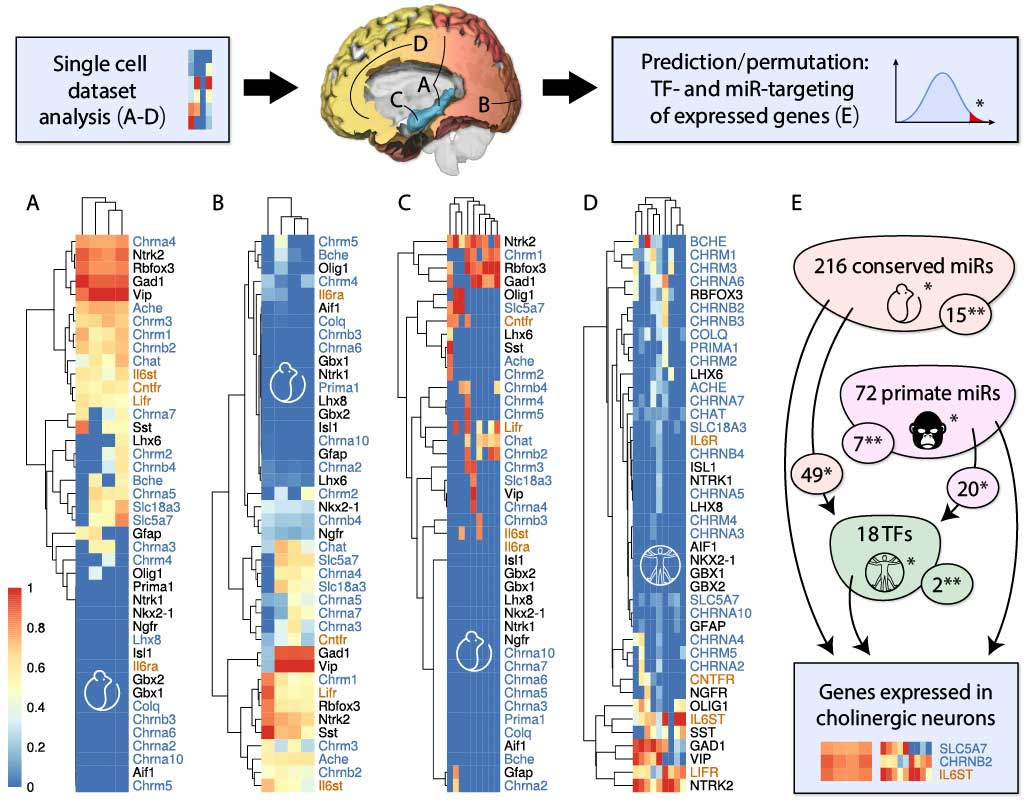
\includegraphics[height=10cm]{figures/singlecell}
\caption[Single-Cell Sequencing of CNS Tissues.]{\textbf{Single-Cell Sequencing of CNS Tissues.} Expression patterns of cholinergic and cholinergic-related genes were analysed using web-available single-cell sequencing datasets. Expression was normalised to reflect a span between 0 and 1. \textbf{A)} Clustered single-cell sequences from transgenic mouse somatosensory cortex and hippocampus.\cite{Zeisel2015} \textbf{B)} Clustered single-cell sequences from transgenic mouse visual cortex.\cite{Tasic2016} \textbf{C)} Single-nucleus sequencing of adult mouse hippocampus.\cite{Habib2016} \textbf{D)} Single-cell sequencing of the human developing neocortex.\cite{Darmanis2015} 
\label{fig:singlecell}}
\end{figure}

The identified samples provide an overview of potentially cholinergic cells in the sampled brain regions, and allow an assessment of the functional type and gene co-expression patterns in central cholinergic cells (Fig.\,\ref{fig:singlecell}). Most cells identified as cholinergic by this definition expressed the general neuronal marker \textit{\acs{rbf}}, also known by its trivial name NeuN, but not the microglial marker \textit{\acs{aif}}. Few cells (or clusters of cells) expressed non-neuronal markers such as \textit{\acs{gfap}} (astrocytes) or \textit{\acs{oli}} (oligodendrocytes), hinting at sparse non-neuronal cholinergic functions. In agreement with my findings, cells or clusters identified as cholinergic by the authors of the respective studies\cite{Zeisel2015, Tasic2016} (also by personal communication with Peter Lönnerberg) had been classified as interneurons and co-expressed a number of known phenotypic neuronal markers, such as \textit{\ac{sst}} and \textit{\ac{vip}}.

The identified cholinergic cells also revealed a constant co-expression with neurokine-related genes, particularly the transmembrane neurokine receptors \ac{lifr} and \ac{ilst}, demonstrating a capacity to receive and process neurokine signals. In contrast, the high affinity receptor for \ac{ngf}, \textit{NTRK1}, is not co-expressed in mature (NeuN-positive) cholinergic neurons in the analysed regions, fundamentally distinguishing these cells from the basal forebrain cholinergic projection neurons.

\section{microRNA and Transcription Factor Targeting Predictions}
\begin{method}
Making use of the information aggregated in \emph{miRNetDB}, the genes identified as being expressed in cholinergic neurons were subjected to permutation targeting analyses of miRNAs and TFs. Genes were assumed to be expressed in cholinergic neurons if they were expressed in more than one individual sample in all single-cell \ac{seq} datasets (Fig.\,\ref{fig:singlecell}\,A-D). The TFs identified as active towards cholinergic genes in cholinergic neurons were additionally subjected to another round of miRNA targeting permutation analysis. Targeting of genes with random selections of miRNAs and TFs were permuted XX times to estimate \ac{fdr}. Statistical significance of the miRNA$\to$gene or TF$\to$gene interactions was assumed at FDR < 0.05.
\end{method}

Permutation targeting analyses revealed a nested regulatory interaction between 72 primate-specific miRNAs, 216 conserved miRNAs, and 18 TFs towards cholinergic genes expressed in cholinergic neurons (Fig.\,\ref{fig:singlecell}\,E). TFs targeting cholinergic genes were in turn targeted by 49 conserved and 20 primate-specific miRNAs that also targeted cholinergic genes directly.

\begin{method}

\section{Gene Clustering Based On Expression}

Hierarchic clustering was applied to expression data to identify functional grouping of genes and cells based on co-expression. Initially, samples (i.e., single cells, pre-aggregated clusters of cells, or brain regions) are compared using a similarity- or distance-matrix (where similarity = \num{1} - distance). The similarity measure is based on a computation according to the method used. For instance, Euclidean distance between two gene expression vectors (i.e., samples) of length $n$ is the distance between points $p$ and $q$ in $n$-dimensional space, defined by: $$d_E(p, q) = \sqrt{\sum_{i=1}^{n} (p_{i}-q_{i})^2}$$

Applying this measure to all pairwise combinations of samples results in a dissimilarity matrix that can be converted to a hierarchy using one of several clustering algorithms. Generally, samples are grouped by their similarity. Initially, each sample is assigned to its own cluster, and then, cluster number is iteratively reduced by joining the closest clusters. This results in a hierarchic tree of samples, that can be »cut« at any height to yield an arbitrary number of clusters. In biological analyses, the method after Ward (in R, »Ward.D2«) is often used.\cite{Murtagh2014}

Due to the structure of the data (small number of entities compared to whole genome analysis, repetition of zeroes in individual samples), the Bray-Curtis dissimilarity\cite{Bray1957} is superior to Euclidean distance. Bray-Curtis dissimilarity is defined as: $$d_{BC}(p, q) = \frac{2C_{p, q}}{S_p+S_q}$$ Where $C$ is the sum of the lesser expression values common to both vectors $p$ and $q$, and $S$ is the total number of genes expressed in each sample (i.e., values greater than zero in each vector). Based on this measure, the samples were clustered according to their cholinergic gene expression levels using Ward's method to yield five separate clusters. Intermediary clustering results (not shown) revealed a uniform distribution of \ac{acly}, yielding no additional information; thus, it was removed. Also removed for the purpose of clustering were the non-neuronal nicotinic receptor subunits $\upalpha$\num{1}, $\upbeta$\num{1}, $\upgamma$, $\updelta$, and $\upepsilon$. 

\end{method}

\subsection{Co-Expression of Functional Groups of Cholinergic Genes}
Hierarchic clustering of cholinergic genes in each of the datasets revealed a grouping of cholinergic genes according to their biological function. Table \ref{tab:chol-clusters} shows considerable uniformity in two single-cell mouse datasets, which diverge substantially from the brain-region- and TF-based human set. Generally, clustering shows separation of at least 3 groups of cells, one of which is the classic \emph{cholinergic} neuron with genes for synthesis and transport of acetylcholine. Due to the frequent co-expression of \emph{\ac{chat}} and \emph{\ac{slc}}, it is safe to assume the \emph{\ac{slc}} as a viable substitute for chat expression and clustering in the FANTOM5 data of Marbach \emph{et al.}\cite{Marbach2016} (for more details, see Section \ref{sec:database:tf}). In the single-cell datasets, the \emph{CHAT} gene is expressed in parallel with the two cholinergic transporters, without exemption. The other groups could be described as \emph{receptive} neuron (not cholinergic as the aforementioned, but different types of cholinergic receptors and esterase) and other, rather specialised groups, probably comprising various glial cells. These last, specialised groups are not very visible in the human dataset, which lacks the single cell resolution of the mouse datasets and therefore includes glial cells in every sample of any region. Therefore, differences in cholinergic gene expression patterns derived from Marbach et al are likely the result of the numbers and dominant types of cholinergic neurons in the respective region.

Functional stratification of cholinergic genes is also visible in a dendrogram of gene clusters from all four analysed single-cell sequencing datasets (Fig.\,\ref{fig:chol-clusters}). While there is variability in the composition of receptor subunits (which is to be expected regarding the different sampled brain regions), the core cholinergic genes (such as \emph{CHAT}, \emph{SLC18A3}, \emph{SLC5A7}, and \emph{ACHE}) associate similarly in all datasets. Notably, the distinction between a \emph{cholinergic} and a \emph{cholinoceptive} neuron is always visible by a grouping of, on one hand the synthesis, vesicular packaging, and reuptake of \ac{ach}, and on the other hand, cholinergic receptors and signal termination by AChE.

\begin{table}[ht]
\sffamily
\small
\centering
\begin{tabular}{c | c | c | c}
cluster & Zeisel et al & Tasic et al & Marbach et al \\
\hline
\hline
I & \makecell{Ache, Chrm1, \\Chrm2, Chrm3, \\Chrm4, Chrna4, \\Chrna5, Chrna7, \\Chrnb2} & \makecell{Ache, Chrm1, \\Chrm2, Chrm3, \\Chrm4, Chrna2, \\Chrna4, Chrna5, \\Chrna7, Chrnb2, \\Chrnb4} & \makecell{CHRM1, CHRM2, \\CHRM5, CHRNA2, \\CHRNA4, CHRNA6, \\CHRNB2, CHRNB3} \\ \hline
Ib&  &  & \makecell{ACHE, BCHE, \\CHRNA3, CHRNB4, \\PRIMA1} \\ \hline
Ic& &  & CHRM3 \\ \hline
Id&  &  & CHRNA5, CHRNA9 \\ \hline
II& \makecell{Chat, Chrnb4, \\Slc18a3, Slc5a7} & \makecell{Chat, Chrm5, \\Chrna3, Slc18a3, \\Slc5a7} & SLC18A3, SLC5A7 \\ \hline
III& \makecell{Chrm5, Chrna10, \\Chrna3} & Chrna10 &  \\ \hline
IV&Bche, Prima1 & Bche, Prima1 &  \\ \hline
V& \makecell{Chrna2, Chrna6, \\Chrnb3} & Chrna6, Chrnb3 &  \\
\end{tabular}
\caption{\textbf{Cholinergic gene clusters according to cell type vs. brain region.} The two transgenic mouse datasets from Zeisel et al and Tasic et al show high similarity in gene distribution. With high likeliness, cluster I is a group of postsynaptically cholinergic, "receptive" cells. Cluster II represents the classic "cholinergic" neuron, with synthesis, vesicular packaging and ACh-reuptake genes. The transcription factor-based dataset of Marbach \emph{et al} depends on whole brain regions instead of single cells to determine similarity, and thus yields distinctly different classification. However, it also distinguishes between cholinergic synthesis (with SLC18A3 as a substitute for CHAT expression) and cholinoceptive functions.}
\label{tab:chol-clusters}
\end{table}

\begin{figure}
\centering
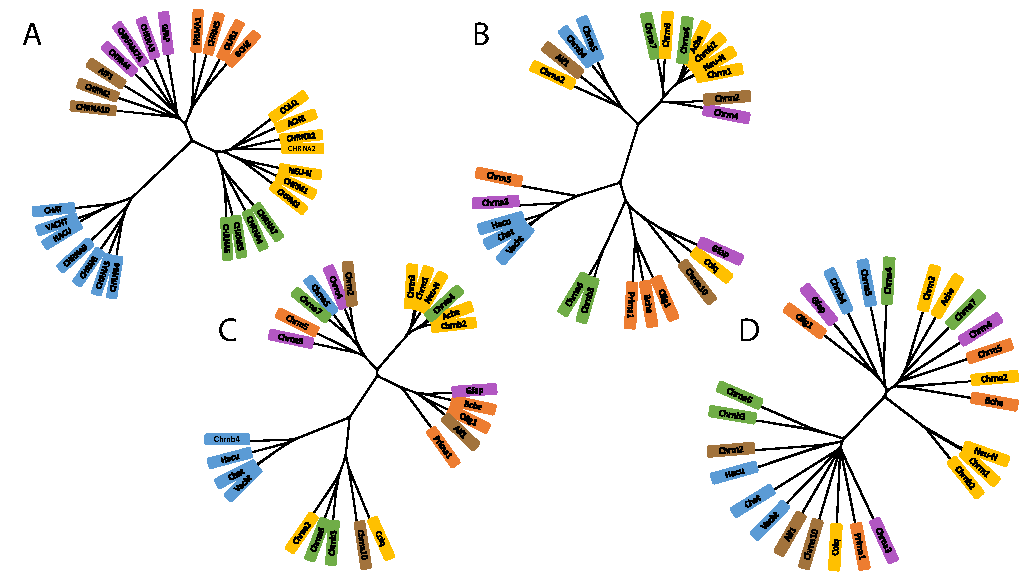
\includegraphics[width=\textwidth]{figures/chol-clusters}
\caption[Clusters of Cholinergic Genes in Single-Cell Sequencing.]{\textbf{Clusters of Cholinergic Genes in Single-Cell Sequencing.} Cholinergic genes were clusteres using Bray-Curtis dissimilarity in four public data sets of single-cell sequencing. The displayed dendrograms visualise the distance between the genes across all samples. Gene clusters were coloured by grouping in Darmanis \emph{et al.}\cite{Darmanis2015} (A). Notably, genes clustered according to their biological function, for instance, CHAT, vAChT and HACU always are closely associated (blue), as are the genes comprising the putative »cholinoceptive« neuron (yellow). \textbf{A)} Single-cell sequencing of the human developing neocortex.\cite{Darmanis2015} \textbf{B)} Clustered single-cell sequences from transgenic mouse visual cortex.\cite{Tasic2016} \textbf{C)} Clustered single-cell sequences from transgenic mouse somatosensory cortex and hippocampus.\cite{Zeisel2015} \textbf{D)} Single-nucleus sequencing of adult mouse hippocampus.\cite{Habib2016} Marker genes are: NeuN - neurons; OLIG1 - oligodendrocytes; AIF1 - microglia; GFAP - astrocytes.
\label{fig:chol-clusters}}
\end{figure}

%!TEX root = ../dissertation.tex
\section{The Cellular Model}
We selected two mono-cultures of human neuronal cells for subsequent experiments: \acs{la2} and \acs{la5}. During the selection process, multiple options were considered. Multicellular models would, in principle, allow disentanglement of the functions of distinct cell types, for instance glia and neurons. This could be achieved by \emph{in vivo} or \emph{ex vivo} approaches in rodents. However, our diseases of interest (Section \ref{sec:intro:diseases}) display a noticeable lack of transferability from lower mammals to human(cite). Alternatively, co-cultures of human cells in mono-layer or as 3D-culture have been proposed, but these still lack experimental stability.

\subsection{The SH-SY5Y Neuroblastoma Cell Line}
A prominent example of human neuronal cell culture used in the identification and elucidation of cholinergic processes is the immortalised neuroblastoma cell line SH-SY5Y.\cite{Biedler1978} Derived from its parent line SK-N-SH, an adrenergic neuroblastoma,\cite{Biedler1973} it expresses ample amounts of \textit{\ac{ache}}, and thus had become a work horse in many cholinergic fields, such as Alzheimer's Disease (which is treated with \ac{achep} inhibitors), pesticide development, and warfare(cite). However, in spite of its usefulness for processes involving \textit{\ac{ache}}, it turned out a less than optimal choice for the study of molecular events surrounding \textit{\ac{chat}} and \textit{\ac{slc}}, as it barely expresses both genes(cite), and cannot be coerced to elevate \textit{\ac{chat}} expression by the usual differentiation techniques (own experimentation, data not shown). Thus, for the questions asked in this chapter of the dissertation, SH-SY5Y does not qualify as adequate representation of a »cholinergic neuron«.

\subsection{The LA-N Neuroblastoma Cell Lines}
Following the elimination of SH-SY5Y as a suitable subject, a literature search for candidates representing a cholinergic neuronal transcriptome revealed, among others, representatives of the LA-N neuroblastoma cell lines developed by R.C. Seeger around 1980.\cite{Seeger1977, Seeger1982} Neuroblastoma is a form of neuronal cancer often affecting small children, and, consequently, the two cell lines used in my experiments are immortalised biopsies of a 3 year old girl (\acs{la2}\cite{Seeger1977}) and of a 4 month old boy (\mbox{\acs{la5}}\cite{Seeger1982}). The decision to use \ac{la2} as initial cellular model was influenced by three factors: it is well described in literature, although most studies had been published in the 1980s and 90s; it expresses substantial amounts of \textit{\ac{chat}} and \textit{\ac{slc}}(cite); and it responds to neurokine-mediated differentiation by assuming a neuronal morphology accompanied by further elevation of \textit{\ac{chat}} and \textit{\ac{slc}} expression. \ac{la5} was not nearly as well described as \ac{la2}, but later added to the experimental roster because of the complementary sex and hints towards cholinergic differentiation under retinoic acid.\cite{Hill1997}

\begin{method}

\subsection{Culture}

\ac{la2} and \ac{la5} are very similar in their culture requirements. They have comparatively high duplication times, which can be lowered by using certain conditions that affect medium composition, nutrition, and CO\textsubscript{2} content. The cells were acquired at DSMZ (Braunschweig, Germany), which recommends keeping them in a 50:50 mixture of \ac{dmem} and \ac{rpmi}, with 20\% \ac{fcs} added. Sometimes, recommendations also suggest Leibovitz's L-15 medium, which is specifically designed for low CO\textsubscript{2} conditions, and others have suggested increased CO\textsubscript{2} levels inside the incubator. A combination of the DSMZ-recommended medium with 8\% CO\textsubscript{2} atmosphere inside a 37°C incubator to accelerate growth to a degree that the cells could be split 1:3 to 1:4 in a weekly cycle. This protocol was used for all further experiments, which were performed between splits 2 to 8 after thawing of a batch from -80°C. All handling during maintenance and experimentation was performed under a laminar flow hood.

\subsection{Differentiation}

Neuronal differentiation of neuroblastoma cell lines has been performed in many instances, utilising a wide variety of differentiation agents such as the very general retinoic acid or 5-bromo-uracil, or very specific reagents, such as the neurokines \ac{il}-6 and \ac{cntf}(cite). LA-N cells have also been described to react to a selection of these substances; however, due to our elevated interest in neurokine mechanisms, we opted for a neurokine-based differentiation protocol. In personal communication, James McManaman revealed that the »\textit{\ac{chat}} development factor« that he had discovered\cite{McManaman1988} was, in fact, \ac{cntf}, which had never been published. Additionally, of the neurokines used for differentiation purposes, \ac{cntf} is best described in literature and easily acquired in dried form from Merck (formerly SigmaAldrich, Darmstadt, Germany). \ac{cntf} was resuspended in pure water to a concentration of \SI{25}{\micro\gram\per\milli\litre} and stored for experimentation in aliquots at -20°C.

LA-N cells are very sensitive to repeated temperature changes (or other handling-related disturbances), which resulted in increased amounts of apoptotic cells following repeated removal from the incubator after seeding or medium changes during the experiment (Lobentanzer, not published). For this reason, the differentiation reagent was only added once, 24h after initial seeding of the cells, and further disturbances avoided until the time of lysis. For the maximum duration of the experiments, 120h from seeding until lysis, the initially supplied medium was sufficient for survival.

Differentiation was performed in regular growth medium without changes in \ac{fcs} content, and \ac{cntf} was added to the medium after an initial growth period of 24h. Cells were seeded into 12-well plates at approximately \num{200000} cells/well, with 1 ml of growth medium. To determine the optimal amount of \ac{cntf} for differentiation, time-dose experiments were perfomed for both cell lines in a range from \SIrange{1}{100}{\nano\gram\per\milli\litre} for several time points during four days. Here, we discovered the first pharmacological difference between \ac{la2} and \ac{la5}: the maximum of their cholinergic response to neurokine stimulation (i.e., an elevation in \textit{\ac{chat}} and \textit{\ac{slc}} transcription) occurs at different concentrations of \ac{cntf}. While \ac{la2} cells respond most strongly to \SI{100}{\nano\gram\per\milli\litre}, \ac{la5} cells show an »inverted u«-type dose response with a maximum around \SI{10}{\nano\gram\per\milli\litre} \ac{cntf} (Fig.\,\ref{fig:time-dose-timeline}\,A). James McManaman, who studied LA-N differentiation thoroughly in the 1990s,\cite{McManaman1991} believes both lines to respond in an »inverted u«-type manner (personal communication); thus, in all likelihood the \ac{la2} response would also diminish at \ac{cntf} concentrations significantly higher than \SI{100}{\nano\gram\per\milli\litre}. Also, CNTF concentrations could likely be significantly lowered by removal of the high amount of \ac{fcs} in the medium, however, that would require the use of a special serum-free medium, which would have to be established up front, and may have other, unforeseen consequences. Regardless, \ac{cntf} concentrations around \SI{100}{\nano\gram\per\milli\litre} (i.e., pico- to nano-molar) still are well within the physiological range of concentrations that the mammalian brain is able to reach by paracrine secretion via, e.g., astrocytes.\cite{Sun2016}\todo{vacht qpcr figure?}

\end{method}

\begin{figure}
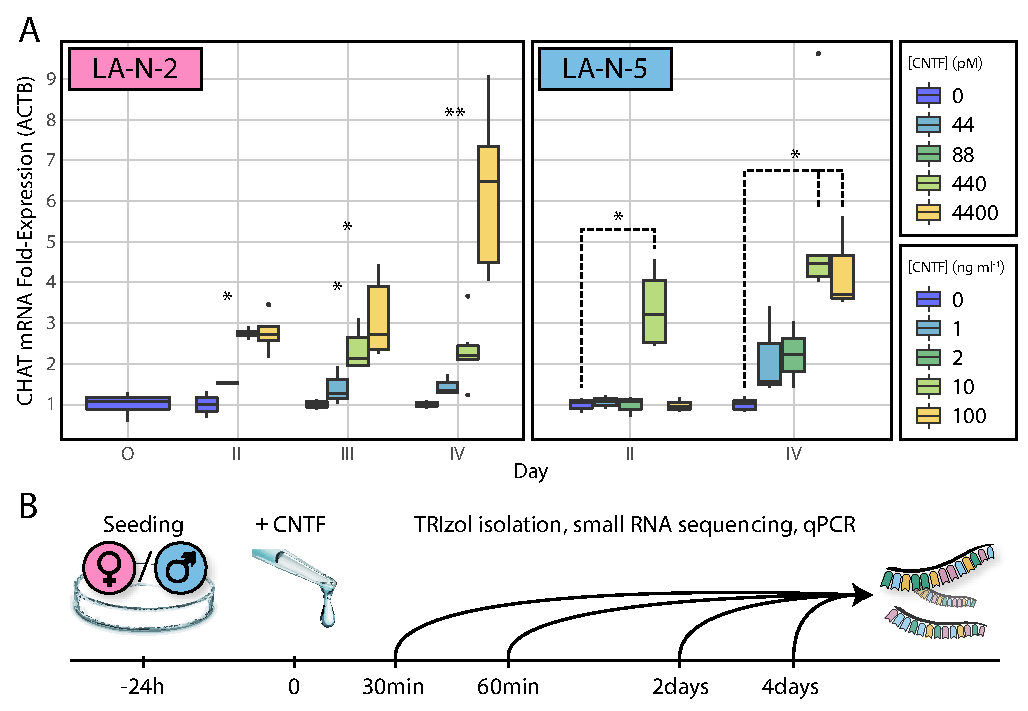
\includegraphics[width=\textwidth]{figures/time-dose-timeline}
\caption[LA-N-2 and LA-N-5, Time-dose Curve and Differentiation Timeline.]{\textbf{Time-dose curve of CNTF-mediated differentiation of LA-N-2 and LA-N-5.} \textbf{A)} Cells were stimulated with varying doses of CNTF, and lysed at various time points to determine CHAT mRNA levels via qPCR. Expression ($\Delta\Delta{C}_t$) was normalised to housekeeping genes (ACTB, GAPDH, RPLP0) and to control sample without CNTF to determine fold-changes. LA-N-5 reacts strongest to a concentration of \SI{10}{\nano\gram\per\milli\litre}, while LA-N-2 reacts strongest to \SI{100}{\nano\gram\per\milli\litre}. *: p < 0.05, **: p < 0.001 \textbf{B)} Cells were seeded at $\smallsim$\e{2}{5} cells/well in a 12-well-plate. After 24h, CNTF was added to the existing medium as quickly as possible to avoid disturbance. Cells were lysed \textit{in situ} at time points 30 minutes, 60 minutes, 48 hours, and 96 hours using TRIzol for downstream RNA processing.
\label{fig:time-dose-timeline}}
\end{figure}

\begin{method}

To study the small RNA dynamics following \ac{cntf} exposure of \ac{la2} and \ac{la5}, the experiment was stopped at 4 time points and the cells were quickly lysed \textit{in situ} to preserve total RNA in that state: for the quick, immediate-early-like phase, at 30 and 60 minutes after the addition of \ac{cntf}, and, for the long-term effects of differentiation, at 48 and 96 hours after the addition of \ac{cntf} (Fig.\,\ref{fig:time-dose-timeline}\,B, from Lobentanzer \textit{et al.}\cite{Lobentanzer2019a}). Each time point was controlled by a pseudo-treated (using pure water) culture from the same batch that had been seeded at the same time as the experimental group. In the final series used for the parallel sequencing of \ac{la2} and \ac{la5}, all experiments were carried out in quadruplicates. 

\subsection{RNA Isolation}

Total RNA was isolated using TRIzol (ThermoFisher Scientific), essentially as suggested by the manufacturer, with slight changes to the protocol to enrich small RNA species. The cells, growing in a monolayer in 12-well-plates, were cleared of medium, washed two times with \SI{500}{\micro\litre} of cell culture grade \ac{pbs} (Gibco), and immediately suspended in \SI{1}{\milli\litre} of TRIzol, pipetting up and down until visibly dissolved. After incubation for 5 minutes at room temperature, the samples were stored in -20°C for short periods of time until RNA isolation.

TRIzol-suspended lysates (\SI{1}{\milli\litre}) were added to RNA-separation centrifuge tubes (PhaseMaker Tubes, ThermoFisher Scientific), adding \SI{200}{\micro\litre} of pure chloroform and mixing vigorously for 15 seconds. After two minutes, the mixture was centrifuged at \SI{12000}{\g} and 4°C for 15 minutes, and the upper, watery phase containing the RNA was extracted. This was mixed with approximately 2 parts of pure ethanol and incubated for 10 minutes at room temperature to precipitate the RNA. The precipitate was spun at \SI{12000}{\g} and 4°C for another 10 minutes, and the supernatant discarded. The pellet was washed with 85\% ethanol (vortexed briefly) and centrifuged again for 5 minutes at \SI{7500}{\g} and 4°C.

After the final centrifugation step, the samples were transferred to the laminar flow hood, and air dried after removal of most of the supernatant via micropipettors. The pellet was allowed to dry almost until completion and resuspended in \SIrange{30}{50}{\micro\litre} pure RNase-free water. RNA concentration was measured at a Nanodrop 2000 instrument (ThermoFisher Scientific) and samples were diluted to a uniform concentration of \SI{100}{\nano\gram\per\micro\litre}. Finally, RNA samples were aliquoted according to later purpose and stored at -80°C.

RNA quality was determined by analysis on a 2100 Bioanalyzer instrument (Agilent) using a nano chip and \SI{1}{\micro\litre} of sample; \ac{rin} was near optimal for all samples (>9).

\section{Small RNA Sequencing and Differential Expression Analysis}
\newthought{For the detection and analysis of small RNA species}, \ac{seq} is the current gold standard method. It allows the mapping of a comprehensive transcriptome and thus is vastly superior to small scale and consecutive methods such as \ac{pcr}, and even the larger scale microarrays. Microarrays, while also potentially allowing a »snapshot« of entire transcriptomes, are limited by the predetermined sequences on the chip. \ac{seq}, on the other hand, is not biased towards any structural property of the sample; this is particularly important in the analysis of small RNA species, since their sequences are very variable (\acp{trf}) and still not completely catalogued (\acp{mir}). Assuming an adequate sequencing depth ($\smallgtrsim$\e{1}{6} reads/sample), \ac{seq} allows a comparison of all expressed small RNA species at once, which is immensely helpful when dealing with processes on the combinatorial scale of \ac{mir} regulation.

\subsection{Sequencing} \label{sec:cellculture:sequencing}

For small RNA sequencing, the aliquoted samples were shipped on dry ice to the cooperating institute at the Hebrew University of Jerusalem, the Silberman Institute of Molecular Biology, the laboratory of Prof. Hermona Soreq. \SI{600}{\nano\gram} of total RNA per sample were prepared for sequencing using the NEBNext Small RNA Library Prep Set for Illumina (New England BioLabs). The libraries were multiplexed with coloured barcodes, allowing for sequencing of all 48 samples on one chip. Briefly, this includes ligation of sequencing adapters to both 3' and 5' ends of all (single-stranded) RNA fragments in the sample, followed by 12-15 cycles of reverse transcription to form the RNA library. Ligated and amplified libraries were then size selected via gel electrophoresis on a 6\% Polyacrylamide gel. The band representing small RNA species on the gel was excised and prepared for loading onto the sequencing chip. After loading, the chip was sequenced in a NextSeq 550 series instrument (Illumina) with a read length of 80 \acfp{nt}, single-end. 

The quantity of reads per sample was determined by analysis of the raw fastq files. The read count across all samples before filtering was \e{7.8}{06} $\pm_{SD}$ \e{2.5}{6}, read count after quality filter and adapter removal was \e{6.8}{6} $\pm_{SD}$ \e{2.2}{6} (n = 48); a mean of 87\% of reads remained after filtering, exceeding the recommended minimum amount ($\smallsim$\num{1} million) by 4- to 12-fold (Fig.\,\ref{fig:read-quality-length}\,A). Overall, $\smallsim$326 million reads remained to be passed down to subsequent analyses. Sequencing quality was determined by analysis of the raw reads using the FastQC software(cite). Even before adapter removal and quality filtering, FastQC detected no »reads of poor quality« in any sample. Fig.\,\ref{fig:read-quality-length}\,B gives a representative example of read quality per base (Sample \num{1}).

\end{method}

\begin{figure}[ht]
\centering
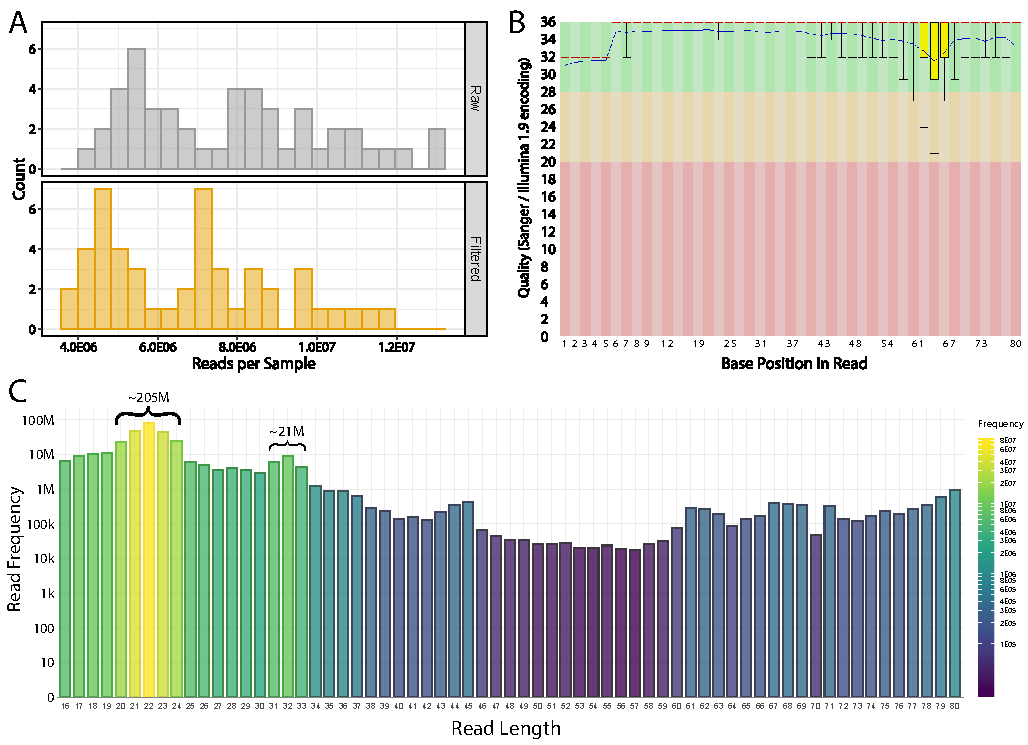
\includegraphics[width=\textwidth]{figures/read-quality-length}
\caption[Small RNA Sequencing - Read Count, Quality, and Length.]{\textbf{Small RNA Sequencing - Read Count, Quality, and Length.} All samples provided near optimal quality. \textbf{A)} Per sample read count had a mean of \e{7.8}{06} $\pm_{SD}$ \e{2.5}{6} in raw samples (top) and \e{6.8}{6} $\pm_{SD}$ \e{2.2}{6} after quality filtering and adapter removal (bottom). 87\% of reads were retained after filtering, with samples spanning read count values between 4 and 12 million. \textbf{B)} Representative example of quality score per base position in the sequencing (FastQC output of sample \num{1}). Quality scores are always near the optimum, with a characteristic slight dip around nt 65. This occurs in all samples and is likely a technical result of the sequencing process. Possibly, it reflects the most common adapter ligation position after size selection of the RNA pool. \textbf{C)} Read length was determined for every one of the $\smallsim$326 million reads. Nearly 80 million reads have a length of 22 nt, and the peak from 21 to 24 nt comprises $\smallsim$205 million reads. This represents the bulk of miRNAs, and probably a significant amount of tRFs. The second peak, from 31 to 33 nt, still comprises $\smallsim$21 million reads; these in all likelihood represent the longer tiRNAs. The reads above a length of 33 nt only sum up to an amount of $\smallsim$6 million, and may contain RNA of viral origin, or even mature tRNAs.
\label{fig:read-quality-length}}
\end{figure}

\begin{method}

Raw reads were adapter-trimmed and quality filtered using the flexbar software\cite{Roehr2017} with parameters

\begin{center}\texttt{-a adapters.fa -q TAIL -qf sanger -qw 4 \\-min-read-length 16 -n 1 --zip-output GZ}\end{center} 

The sequence used in the \textit{adapters.fa} file, as recommended by the manufacturer, was $$AGATCGGAAGAGCACACGTCTGAACTCCAGTCAC$$ 

Paired-end sequencing still is superfluous in small \ac{seq}, because none of the common alignment pipelines can use the second (reverse) read, and manual paired alignment does not yield nearly as much benefit as the depth increase in single-end sequencing (the read count per sample effectively doubles). 80 \acp{nt} is the maximum read length possible in our small RNA workflow, and is excessive for the analysis of \acp{mir}. For \aclp{trf}, however, a longer read can yield a more complete picture of expression, since the longer \acp{tirna} can easily reach 40 \acp{nt} in length. Indeed, the read length distribution after adapter removal shows a significant amount of small RNA species exceeding the length possible for \acp{mir} (Fig.\,\ref{fig:read-quality-length}\,C).  \todo{align longer reads to genome? viral?} \todo{discuss in text?}

\end{method}

%\begin{figure}
%\centering
%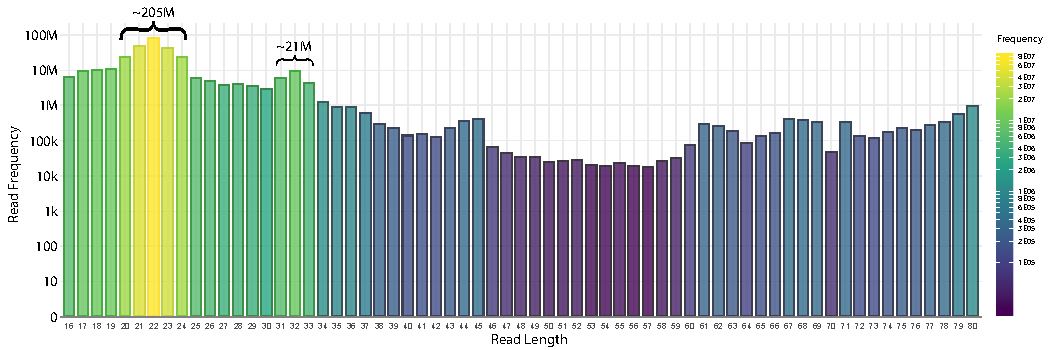
\includegraphics[width=\textwidth]{figures/read-dist-after-flexbar}
%\caption[Small RNA Sequencing - Read Distribution after Trimming and Filtering.]{\textbf{Small RNA Sequencing - Read Distribution after Trimming and Filtering.} Read length was determined for every one of the $\smallsim$326 million reads. Nearly 80 million reads have a length of 22 nt, and the peak from 21 to 24 nt comprises $\smallsim$205 million reads. This represents the bulk of miRNAs, and probably a significant amount of tRFs. The second peak, from 31 to 33 nt, still comprises $\smallsim$21 million reads; these in all likelihood represent the longer tiRNAs. The reads above a length of 33 nt only sum up to an amount of $\smallsim$6 million, and may contain RNA of viral origin, or even mature tRNAs.
%\label{fig:read-dist-after-flexbar}}
%\end{figure}

\begin{method}

\subsection{Sequence Alignment} \label{sec:cellculture:alignment}

For the alignment of \ac{mir} sequences, parts of the miRExpress 2.0\cite{Wang2009} pipeline were used according to the documentation. First, a lookup table for the current miRBase version 21 was created as per the instructions of the authors. The alignment was then performed using the commands \textit{Raw\_data\_parse}, \textit{statistics\_reads}, \textit{alignmentSIMD}, and \textit{analysis}; \textit{Trim\_adaptor} \todo{describe what miRExpress does?} was skipped because the adapters had already been trimmed in the quality filtering step. Additionally, since miRExpress is not accepting of sequences of any length, the raw data was length filtered to include only reads up to a length of 25 \acp{nt} before input into miRExpress. Thus, raw reads were aligned to the miRnome provided by miRBase v21, yielding count tables of mature \acp{mir} and miRNA precursors for each sample. In total, 1913 mature \acp{mir} from miRBase v21 were discovered in the data.

\subsection{Differential Expression Analysis - R/DESeq2} \label{sec:cellculture:deseq}

To determine the effect and dynamics of \ac{cntf}-mediated differentiation of \ac{la2} and \ac{la5}, the expression state of each measured time point was compared to the respective control using the established R package \textit{DESeq2}.\cite{Love2014} \textit{DESeq2} determines differential expression (for gene $i$ and sample $j$) in count-based data by application of a linear regression model to a negative binomial distribution based on a fitted mean $\mu_{ij}$ and a gene-specific dispersion value $\alpha_i$. The mean is derived using a sample-specific »size factor«, $s_j$, and a parameter $q_{ij}$ proportional to the expected true concentration of RNA fragments in the sample. The \textit{DESeq2} differential expression pipeline is composed of the following commands:
\begin{itemize}[noitemsep, leftmargin=.5cm, label={\tiny\raisebox{1ex}{\textbullet}}]
\item \texttt{estimateSizeFactors()} to estimate $s_j$
\item \texttt{estimateDispersion()} to estimate $\alpha_i$
\item \texttt{nbinomWaldTest()} application of a generalised linear model to determine log-fold changes and statistics via the Wald test, using $\mu_{ij} = s_jq_{ij}$ and $log_2(q_{ij}) = x_j\beta_i$.
\end{itemize}
The Wald test, named after Abraham Wald,\cite{Wald1939} is an approach to hypothesis testing that measures the distance between the tested unrestricted estimate and the null hypothesis, using the precision as a weighting factor. The larger the distance between tested values and the null, the more likely the measured values are »true«. \ac{seq} data can be modelled using binomial distributions,\cite{Bullard2010} such as the Poisson distribution, and the difference between two Poisson means (e.g., »treated« vs »control«) can be tested by generalised linear models based on the distributions directly (Poisson regression), Fisher's exact test, or the likelihood ratio test. However, comparative analysis has shown that the Wald test on log-transformed data provides statistical power superior to these other methods,\cite{Chen2011} particularly in lowly expressed fragments. The design formula for the linear regression was applied to \ac{la2} and \ac{la5} separately as a simple factor combination of condition and time point: $$y \smallsim condition\_time$$

The heteroskedastic nature of \ac{seq} count data (variance is much higher in low-count features) brings statistical problems. To reduce the noise introduced by the high variance in low-count genes while preserving large, »real« differences, the authors propose the »shrinkage« of log-fold changes to avoid arbitrary low-cut filtering at a predefined expression (count) value. Multiple variants are available; for \ac{mir} data, the adaptive algorithm »apeglm«\cite{Zhu2019} (adaptive t prior shrinkage estimator) yielded sensible results (see Fig.\,\ref{fig:apeglm-comp-la2d4}).

\end{method}

\begin{figure}[ht]
\centering
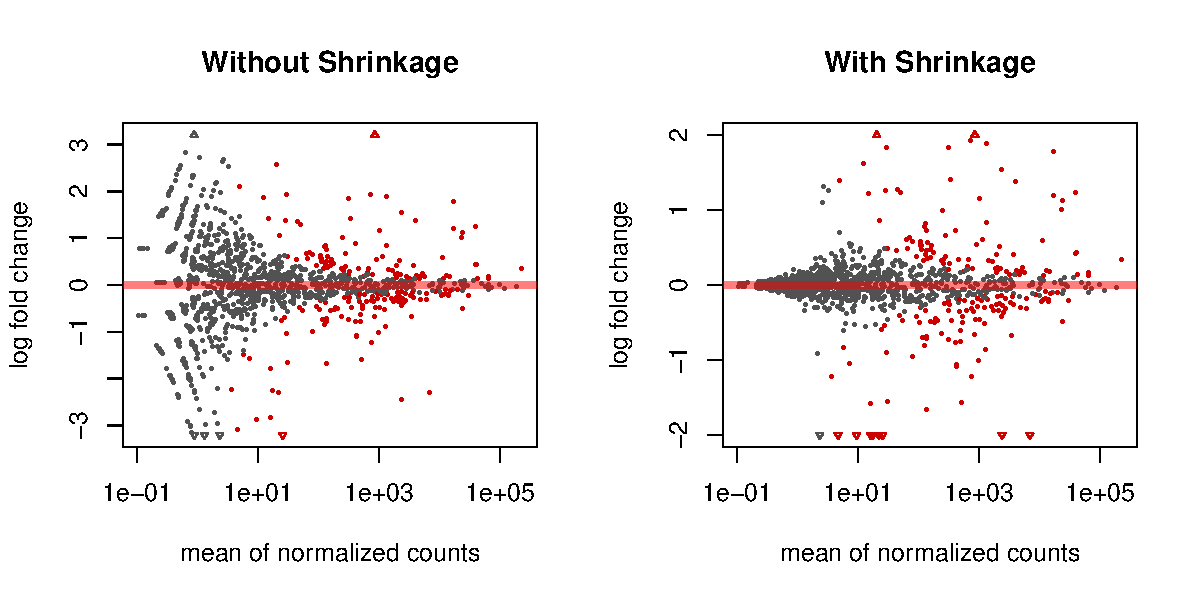
\includegraphics[width=\textwidth]{figures/apeglm-comp-la2d4}
\caption[MD Plot Shrinkage Comparison.]{\textbf{MD Plot Shrinkage Comparison.} A mean-difference plot (MD Plot) is a plot of log-intensity ratios (differences, »M-values«) versus log-intensity averages (means, »A-values«); it is synonymous with »MA Plot«. The \textit{DESeq2} function \textit{plotMD} shows the fold changes attributable to a given variable over the mean of normalised counts for all the samples in the data set. Points will be coloured red if the adjusted p value is less than 0.1. Points which fall out of the window are plotted as open triangles pointing either up or down. The left plot is generated from the standard linear model, the plot on the right is corrected by the »apeglm« algorithm\cite{Zhu2019} to reduce noise in the low-count fragments (data from \ac{la2} \ac{cntf} vs control on day 4).
\label{fig:apeglm-comp-la2d4}}
\end{figure}

\subsection{microRNA Dynamics in CNTF-mediated Cholinergic\\ Differentiation of LA-N-2 and LA-N-5}
Differential expression analysis performed in this manner yielded 490 \ac{de} \acp{mir} across all groups, with characteristic distributions between cell lines and time points. The raw data and processed counts were deposited to \ac{ncbi} \ac{geo}, accession GSE132951. An earlier sequencing experiment (deposited as GSE120520), which was similar in principle, but only comprised three biological replicates and only \ac{la2}, reproduced 80\% of \ac{de} \acp{mir} in the newer \ac{la2} samples. Considering the general reproducibility of \ac{seq} and the lower replicate number, 80\% is an excellent substantiation of the result. About 25\% of miRNAs predicted in single-cell permutation targeting analysis (see Fig. \ref{fig:singlecell}\,E) were found DE in LA-N-2 and LA-N-5 (Fig. \ref{fig:cc-cor-de-perm}\,A) in all three groups, i.e., conserved, primate-specific, and TF-targeting miRNAs.  

\subsubsection{Differential Expression in Both Cell Lines}

%\begin{wrapfigure}{r}{0.5\textwidth}
%  \begin{center}
%    \includegraphics[width=0.48\textwidth]{birds}
%  \end{center}
%  \caption{Birds}
%\end{wrapfigure}

114 mature \acp{mir} were detected as \ac{de} in both cell lines, with some changes similar in both, while others were inverted (Fig.\,\ref{fig:cc-cor-de-perm}\,B). In both cases, however, count-change values (see Box \ref{box:count-change}) correlated highly between the two cell lines (similar: 76 \acp{mir}, Spearman’s $\rho = 0.9066$, p < 2.2E-16; inverted: 38 \acp{mir}, $\rho = 0.9294$, p < 2.2E-16).

\begin{figure}[ht]
\centering
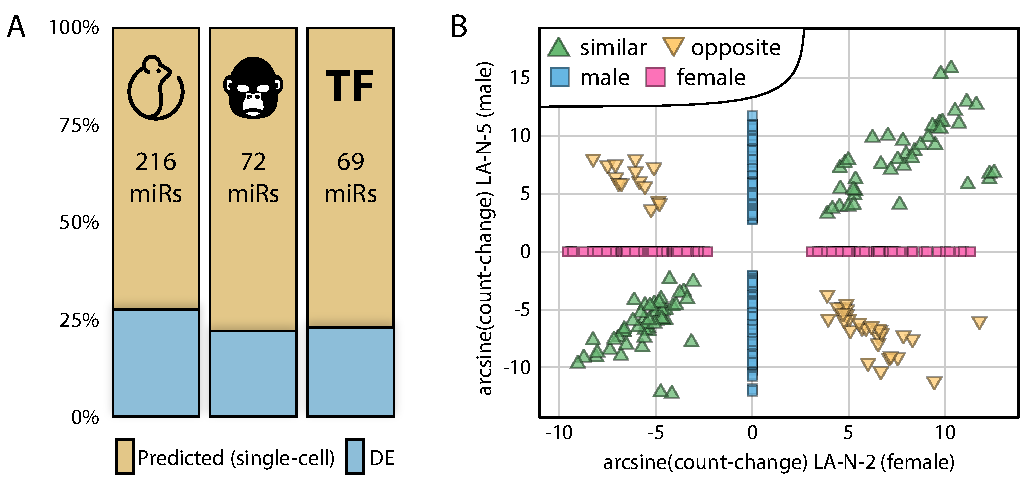
\includegraphics[width=\textwidth]{figures/cc-cor-de-perm}
\caption[Differentially Expressed microRNAs in LA-N-2 and LA-N-5.]{\textbf{Differentially Expressed microRNAs in LA-N-2 and LA-N-5.}
\label{fig:cc-cor-de-perm}}
\end{figure}

\begin{mybox}{The count-change metric}\label{box:count-change}
The frequently used log-fold change metric is not ideally suited for assessing the potential effect of expression changes for individual \acp{mir} because it does not reflect mean expression levels. To determine the absolute change in expression, the count-change metric was introduced, a combination of base mean expression and log-fold change, to weigh DE miRNAs against one another. The count-change is defined as follows: $$CC = (BM \cdot 2^{LFC}) - BM$$
CC: count-change, BM: base mean expression, LFC: log-2-fold-change.

Importantly, by using the base mean expression, count-change correlates directly with sequencing depth. Generalisation, e.g. comparison between two individual experiments, is therefore not straightforward. A normalisation to raw reads would enhance comparability, however, other effects such as fragment distribution and quality aspects may also play a significant role.
\end{mybox}

\subsubsection{Differential Expression Along The Timeline} \label{sec:cellculture:along}
For consistency, from hereon out, time points 30 minutes and 60 minutes will be termed »early«, while 2 days and 4 days will be referred to as »late«. Differential expression was detected in all groups, lending credibility to the rapid changes in expression needed for a \ac{mir} response of the »immediate-early« type. However, the response to long-term \ac{cntf} stimulation was larger in \ac{mir} numbers as well as effect sizes (Fig.\,\ref{fig:timepoints-expr-venn}\,A\&B). Of all early perturbed \acp{mir}, only 3 and 13 \acp{mir} were exclusively perturbed immediate-early-like in \ac{la2} and \ac{la5}, respectively; all others were still \ac{de} after 2 and/or 4 days. In \ac{la2}, the late time points at 2 and, particularly, 4 days showed the greatest perturbation; in \ac{la5}, the picture was more complex (Fig.\,\ref{fig:timepoints-expr-venn}\,C\&D). However, generally, there were large similarities as well as exclusivities between the time points 2 and 4 days in both cell lines. When comparing early and late time points between \ac{la2} and \ac{la5} directly, similarly complex patterns emerged (Fig.\,\ref{fig:timepoints-expr-venn}\,E\&F). Particularly at late time points (Fig.\,\ref{fig:timepoints-expr-venn}\,F), every possible combination of overlap exists. 24\todo{something special?} \acp{mir} were \ac{de} in all late conditions; 107 \acp{mir} were \ac{de} only in \ac{la2}, and 269 \acp{mir} were \ac{de} only in \ac{la5}. \todo{compare most important targets early/late}

\begin{figure} 
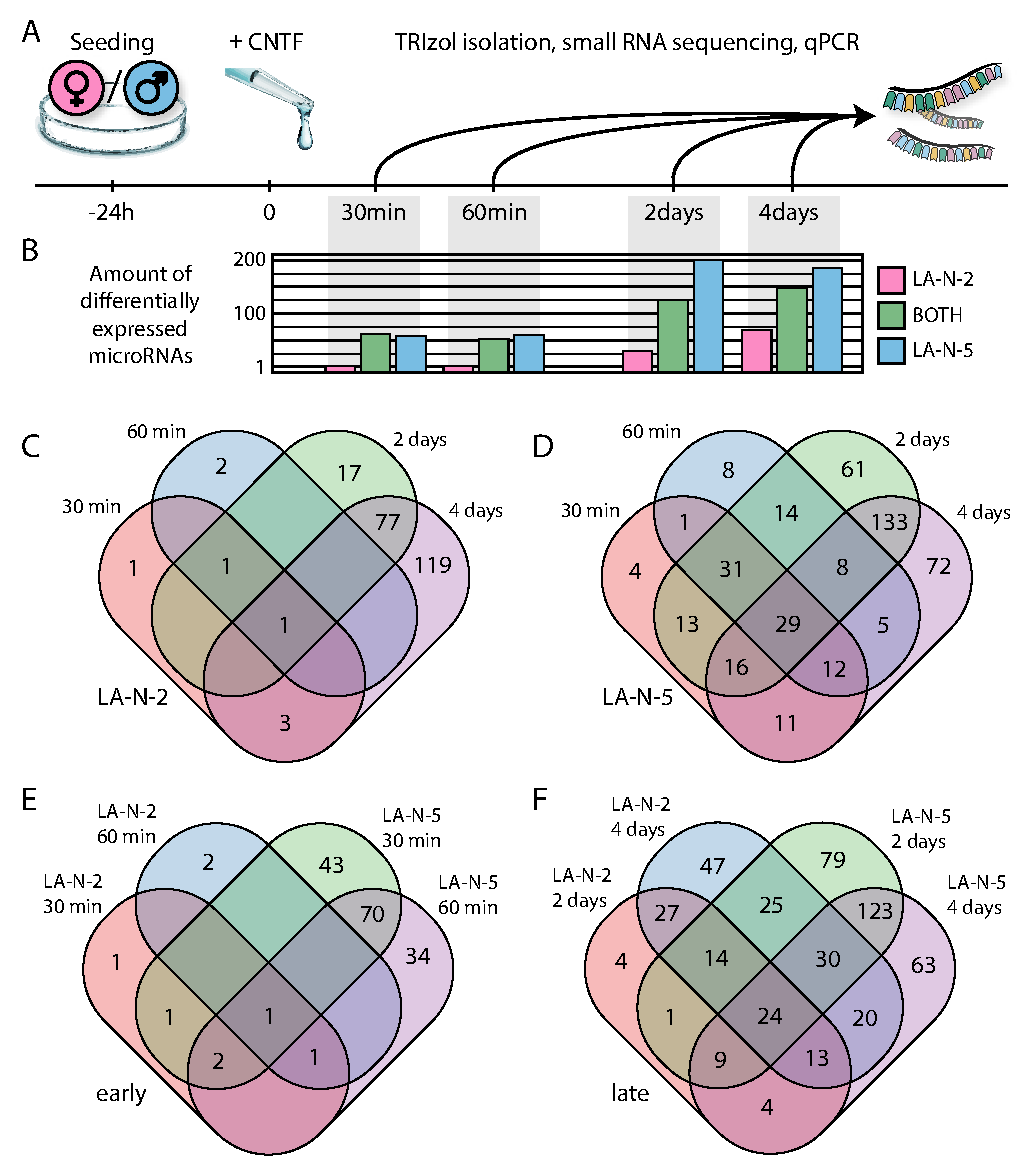
\includegraphics[width=\textwidth]{figures/timepoints-expr-venn}
\caption[Timeline Differential Expression.]{\textbf{LA-N-2 / LA-N-5 Timeline and Differential Expression.} \textbf{A)} Experimental timeline of CNTF differentiation. \textbf{B)} Bar plot of \acf{de} \acp{mir} per time point, divided by cell line where differential expression was measured (\ac{la2} only, \ac{la5} only, or both). \textbf{C)} Venn diagram of \ac{de} \acp{mir} in \ac{la2}, divided by time point. Few early \ac{de} miRNAs, and continually more the longer differentiation lasts. \textbf{D)} Venn diagram of \ac{de} miRNAs in \ac{la5}, divided by time point. Similar in pattern to \textbf{C}, but more pronounced in number. \textbf{E)} Intersection of early time points in \ac{la2} and \ac{la5}. Despite the low differential expression in \ac{la2}, there is overlap. \textbf{F)} Intersection of late time points in \ac{la2} and \ac{la5}. Overlap is pronounced and complex, however, there are also cell line exclusive \acp{mir}.
\label{fig:timepoints-expr-venn}}
\end{figure}

\subsubsection{Differential Expression Between LA-N-2 and LA-N-5}
While there was considerable intersection in \ac{de} \acp{mir} between the cell lines, a substantial amount of \acp{mir} was only \ac{de} in one of the two lines. Generally, response to \ac{cntf} was higher in the male-originated \ac{la5} cells; however, there were also \acp{mir} found \ac{de} only in the female \ac{la2} (compare Fig.\,\ref{fig:timepoints-expr-venn}). Thus, not all of the differences in \ac{mir} expression can be attributed to a higher sensitivity in \ac{la5}. Similarly, \ac{la5} shows a »non-significant trend« toward higher count-change values (mean of absolute count-change across all DE time points, \num{20907} versus \num{3066}, Welch two-sample t test, p = 0.08).

The influence of genotype on the differentiating effect of \ac{cntf} was determined via a statistical interaction design in the \textit{DESeq2} Wald test. Briefly, by including an interaction term in the linear regression formula, the effect of the condition (\ac{cntf} or control at each time point) between the two genotypes can be isolated: $$y \smallsim condition + genotype + condition:genotype$$

Using the interaction term $condition:genotype$, \acp{mir} that reacted significantly different to \ac{cntf} stimulation in \ac{la5} compared to \ac{la2} were determined. Of note, the sexual dimorphism becomes more pronounced over the course of differentiation. While there is no significant difference between \ac{la2} and \ac{la5} at 30 minutes and only one \ac{mir} \ac{de} at 60 minutes, numbers increase at 2 days and reach a maximum at 4 days, with significant overlap (Fig.\,\ref{fig:la2-vs-la5-overlap-venn}\,A). Although not all miRNAs found in this manner belong to the group of miRNAs with inverted expression between LA-N-2 and LA-N-5, several show significant differential regulation between the male and female cellular models (e.g., hsa-miR-615-3p, Fig.\,\ref{fig:la2-vs-la5-overlap-venn}\,B). To further examine the effect of genotype on the small RNA response to \ac{cntf}, the regular differential expression results (Section \ref{sec:cellculture:along}) were intersected with the interaction term for the late time points. This resulted in a complex pattern of intersecting \acp{mir}, in both cell lines (Fig.\,\ref{fig:la2-vs-la5-overlap-venn}\,C\&D). Again, all possible overlaps between any two groups exist; 37 and 36 \acp{mir} are found in all four groups of \ac{la2} and \ac{la5}, respectively. Among those, 16 mature \acp{mir} belong to all sets. All pertinent sets of \acp{mir} can be found in Appendix \ref{appendix:de-mirs}. \todo{target, GO for which?}

\begin{figure}
\centering
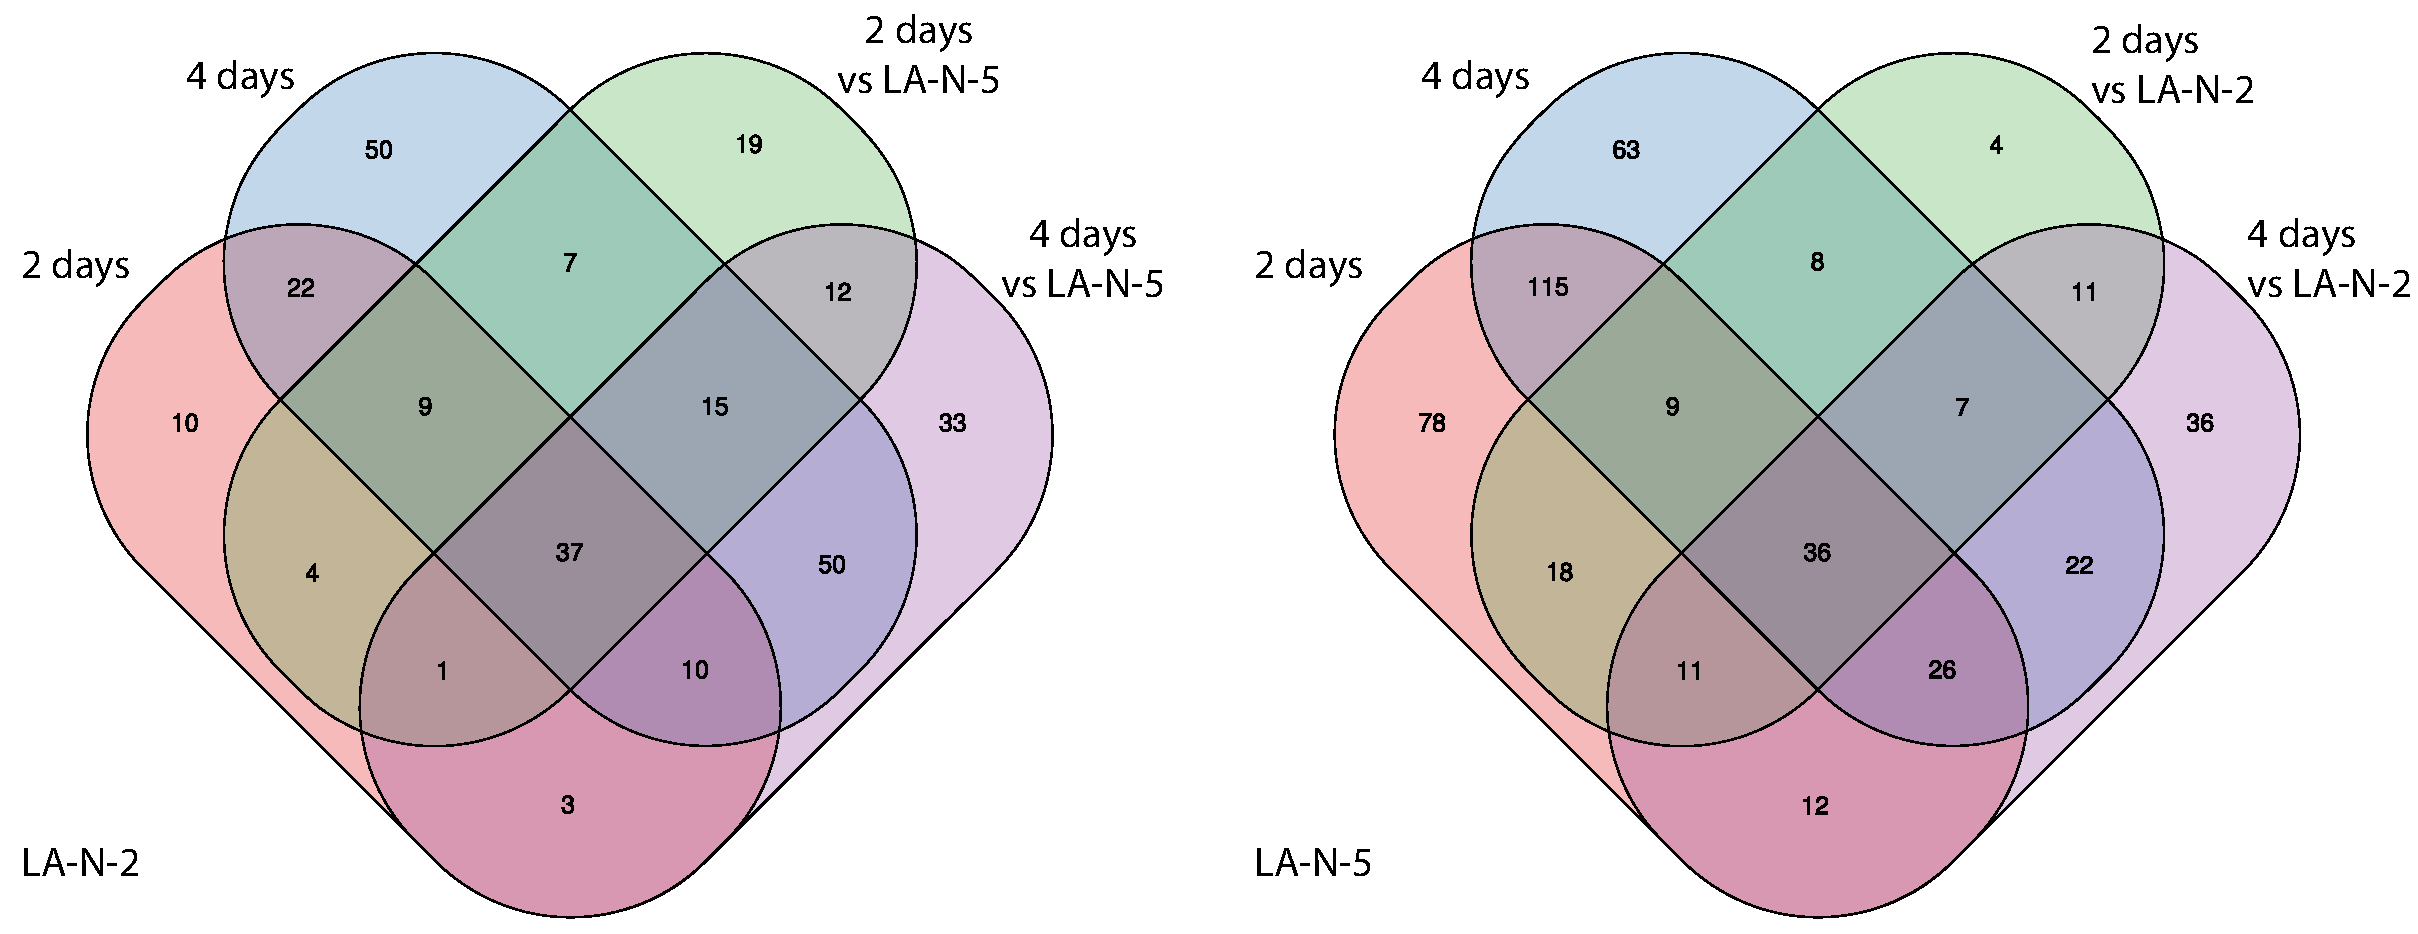
\includegraphics[width=\textwidth]{figures/la2-vs-la5-overlap-venn}
\caption[miRNAs DE between LA-N-2 and LA-N-5.]{\textbf{miRNAs DE between LA-N-2 and LA-N-5.} Application of a design model formula which includes an interaction term enables display of the influence of the male or female genotype on differential miRNA expression. \textbf{A)} Venn diagram of miRNAs differentially expressed \emph{between} LA-N-2 and LA-N-5 at all four time points. \textbf{B)} Counts plot of normalised raw expression values of hsa-miR-615-3p. Exemplary of a high influence of genotype on the differential expression caused by CNTF differentiation, hsa-miR-615-3p is more highly expressed in the female LA-N-2 and elevated after four days of CNTF-induced differentiation, while in the male LA-N-5, it is expressed slightly lower and suppressed upon differentiation. \textbf{C)} Venn diagram comparing late differential expression in LA-N-2 with late time points of differential expression between LA-N-2 and LA-N-5. All possible combinations exist, however, there are miRNAs affected by genotype that are not differentially expressed in the simple model. \textbf{D)} Venn diagram comparing late differential expression in LA-N-5 with late time points of differential expression between LA-N-2 and LA-N-5. Essentially similar to C), but with partly higher quantities of DE miRNAs.
\label{fig:la2-vs-la5-overlap-venn}}
\end{figure}

\subsection{microRNA Family Enrichment}
To categorise and systematise the sexual dimorphism of \ac{cntf} differentiation of LA-N cells, statistically over-represented \ac{mir} families in the differential expression datasets were determined.\todo{how many DE miRs in families?} Of the 151 \ac{mir} families listed in miRBase v21, members of 71 families are \ac{de} in \ac{la2} and \ac{la5}. Enrichment of male, female, and ubiquitously \ac{de} \acp{mir} in these families was determined via hypergeometric gene set enrichment based on Fisher's exact test for each of the families. Five families were enriched in both male and female cells, and 12 families in only one of the two cell lines (Fig.\,\ref{fig:mir-de-fam-go}\,A, left side). The size range of enriched families was substantial, from small families with only 4 mature members to extensive families with dozens of mature \acp{mir}. \todo{which/how many of the pertinent mirs above are in families?}

\subsubsection{Gene Targeting of Enriched Families}
The targets of all individual \acp{mir} in the enriched families were determined via \textit{miRNeo} query. Of note, the amount of family members in any \ac{mir} family did not correlate with the absolute amount of targets predicted (Fig.\,\ref{fig:mir-de-fam-go}\,A). Rather, the influence of individual \acp{mir} was the main factor determining the size of the gene target network. However, those families that were enriched in only one cell line presented with significantly smaller target sets than those that were found \ac{de} in both (mean targeted genes per \ac{mir} 217 versus 378, Welch two-sample t test, p = 0.001). Relative to family size, 4 of the enriched families targeted less genes than all others: mir-10 (p = 0.016), mir-192 (p = 0.042), mir-379 (p = 0.011), and mir-515 (p < 0.001). Hypothetically, the spectrum of target amounts may correlate with the degree of functional specification of distinct \ac{mir} families: on one end, broadly acting families such as let-7 with sex-independent function, on the other, families with a narrow target profile, such as mir-10, whose restricted function can associate with sex-specific effects.

\begin{figure}
\centering
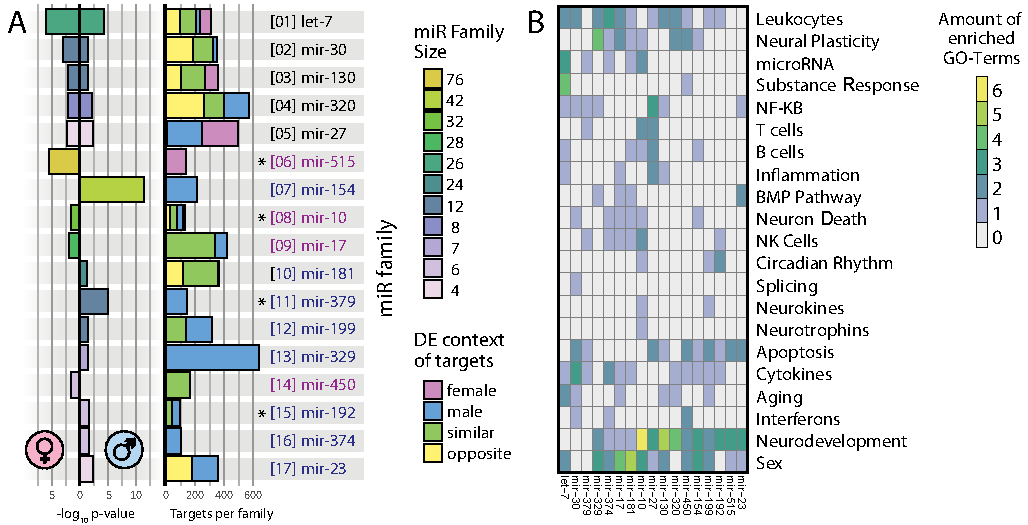
\includegraphics[width=\textwidth]{figures/mir-de-fam-go}
\caption[Differential Expression miRNA Family Enrichment]{\textbf{miRNA Families Enriched in Differential Expression and their Ontological Associations.} 17 miRNA families were enriched significantly in the DE miRNAs following CNTF-mediated differentiation of LA-N-2 and LA-N-5 (Fisher's exact test, p < 0.05). \textbf{A, left side)} Bar plot of p-values of enriched families, ordered by family size; family size encoded by colour. \textbf{A, right side)} Stacked bar plot of the number of gene targets per family. Bars are divided by the DE pattern between LA-N-2 and LA-N-5 of each individual family member. DE context (encoded by colour) varies from detection in all categories (such as let-7 or mir-10) to detection only in one cell line (such as mir-515 or mir-154). Four families show significantly less target genes than all other families in relation to their size (denoted by asterisks). \textbf{B)} Gene Ontology enrichment analysis of gene targets of all enriched families, 737 distinct terms curated into CNS- or immunity-related categories. Families mir-10 and mir-199 show association with neurokines and circadian rhythm.
\label{fig:mir-de-fam-go}}
\end{figure}


%!TEX root = ../dissertation.tex
\section{microRNA Family Gene Ontology Enrichment}
A significant drawback of the recency of the discovery of regulatory small RNAs is the lack of comprehensive functional annotation. While protein coding genes are well annotated and neatly organised into an enormous amount of ontological categories (see Section \ref{sec:database:gsea}), \acp{mir} have only been anecdotally associated with specific functions in the cell. Additionally, the functional roles of protein coding genes are much more limited than those of \acp{mir}; the number of potential functions of any \ac{mir} correlates with the number of mRNA targets this \ac{mir} has, and is also highly context-dependent (e.g. regarding cell type, cell state, disease). Thus, to systematically screen a large amount of \acp{mir} and families, I had to turn to an indirect approach: the \ac{go} analysis of targeted genes.

\begin{method}

\subsection{Creation of miRNA Family Gene Target Sets}
\ac{go} analysis of the targets of a single \ac{mir} is challenging, because the analysis requires a weighted scoring system of input genes. For single \acp{mir}, the options for scoring are limited to the aggregated targeting score or permutation p-values. Using families enables the introduction of a further scoring method: the aggregation of individual family members targeting the same gene. The reasoning behind this approach is to determine a general functional »area« of biological process that the \ac{mir} family in question operates in. To account for the possibility of multiple areas being affected by a family, the test set of genes in any \ac{go} enrichment analysis should not be too small (i.e., rather the top 100 genes than the top 10). 

Following this reasoning, the targets of all \acp{mir} in each family were determined via \textit{miRNet} query. For each family, genes were ranked by their cumulative targeting score $\rho$ from all family members. For gene $i$ and number of \acp{mir} in family $x$, gene score $\rho$ is calculated from individual \ac{mir}$\to$gene scores $s$: $$\rho_{i} = \sum_{n=1}^{x} s_{ni}$$

\subsection{GO Analysis of Target Sets} \label{sec:cellculture:topgo}
The gene target sets of individual \ac{mir} families were ordered decreasingly by their cumulative score $\rho$ and subjected to \ac{go} analysis via the R package \textit{topGO}\cite{Alexa2006}. Briefly, \textit{topGO} analysis extends the basic hypergeometric approach of \ac{go} enrichment analysis by de-correlating the \ac{dag} structure of GO annotation (see Section \ref{sec:database:gsea}), allowing a weighted correction for the interdependency of neighbouring GO nodes. If a gene is found in both the parent node (more general) and the child node (more specific), the less specific parent node gene is weighted less; in this way, the most specific node of each hierarchical branch can be found without confounding the result with less specific terms. While GO analysis always is subject to interpretation by the researcher, this weighted algorithm has been shown to reduce false positives while retaining a high true positive ratio.

\textit{topGO} analysis was performed using the classic (i.e., Fisher's exact test) as well as weighted methods for comparison, however, to determine significance, the p-values calculated by the enhanced weighted algorithm were used. \ac{fdr} was controlled at 5\%. As recommended by the authors, the ordered list of gene targets up to the 3000th position was used as a background for the analysis; the test set in each case was the top 10\% of targeted genes.

\end{method}

\subsection{Large Scale GO Term Curation}
The GO analysis performed in this manner for all 17 enriched families resulted in a list of 737 distinct GO terms related to any of the families. To generate an overview of functional implications of the individual families, the GO terms were filtered and aggregated manually. Terms not relating to CNS- or immune-function were removed, and the remaining terms were sorted into one of 21 categories (Fig.\,\ref{fig:mir-de-fam-go}\,B). Generally, the families associated with neurodevelopment and neural plasticity, diverse immune functions, cell cycle control, and sex. More general categories were found in most families, while more specific functions showed a sparser distribution.

Only two families associate significantly with neurokine-related function, mir-10 and mir-199. Both are involved in neurodevelopment- and sex-related function, and show the very specific association with circadian rhythm. Family mir-10 additionally is implicated in control of neurotrophin-related mechanisms, and in several blood-borne immune cells, such as T-, B-, and NK-cells.

\section{Whole Genome miRNA$\to$Gene Network Generation} \label{sec:cellculture:network}
A common approach to complex network relationships is physical modelling. A complex graph (with directed and weighted edges) can be coerced to self-organise by application of a force-directed layout. In this process (also known as spatialisation), the network, defined only by its nodes and edges, is transformed into a map, usually in two dimensions. An important prerequisite is the scale-free topology of the network, a structure that transcriptional connectomes usually present with(cite). A force-directed layout transforms a network by simulating a gravitational system, or a system of magnetic nodes connected by springs, in which the nodes repel each other, but edges between two nodes pull them towards each other. By manipulation of multiple physical attributes of the model, a mapped representation of the network's organisation can be produced. As a result, nodes (i.e., genes, TFs, and miRNAs) with close interaction are mapped in close proximity, while nodes with low interaction are far apart. Similarly, nodes with pivotal function in the network (»hubs«) gravitate towards the centre of the map, while »less important« nodes are shifted towards the fringes.

\begin{method}

The network comprising all \ac{de} members of the 17 enriched miRNA families and \num{12495} targeted genes as determined via \textit{miRNet} query was subjected to force-directed mapping using the Java-based software Gephi 0.9 and its primary force-directed algorithm, ForceAtlas2\cite{Jacomy2014}. Gephi, and ForceAtlas2, are designed to generally handle graphs with up to \num{10000} unique relationships; however, the standard \textit{miRNet} query resulted in a network with $\smallsim$\num{160000} edges. To reach a computationally manageable number of relationships, the score threshold was raised to a minimum of 7, which resulted in a network of \num{46937} unique edges. The resulting network was exported as a vector graph and manually edited in Adobe Illustrator to further enhance its readability (Fig.\,\ref{fig:bignet}).

\end{method}

\begin{figure}
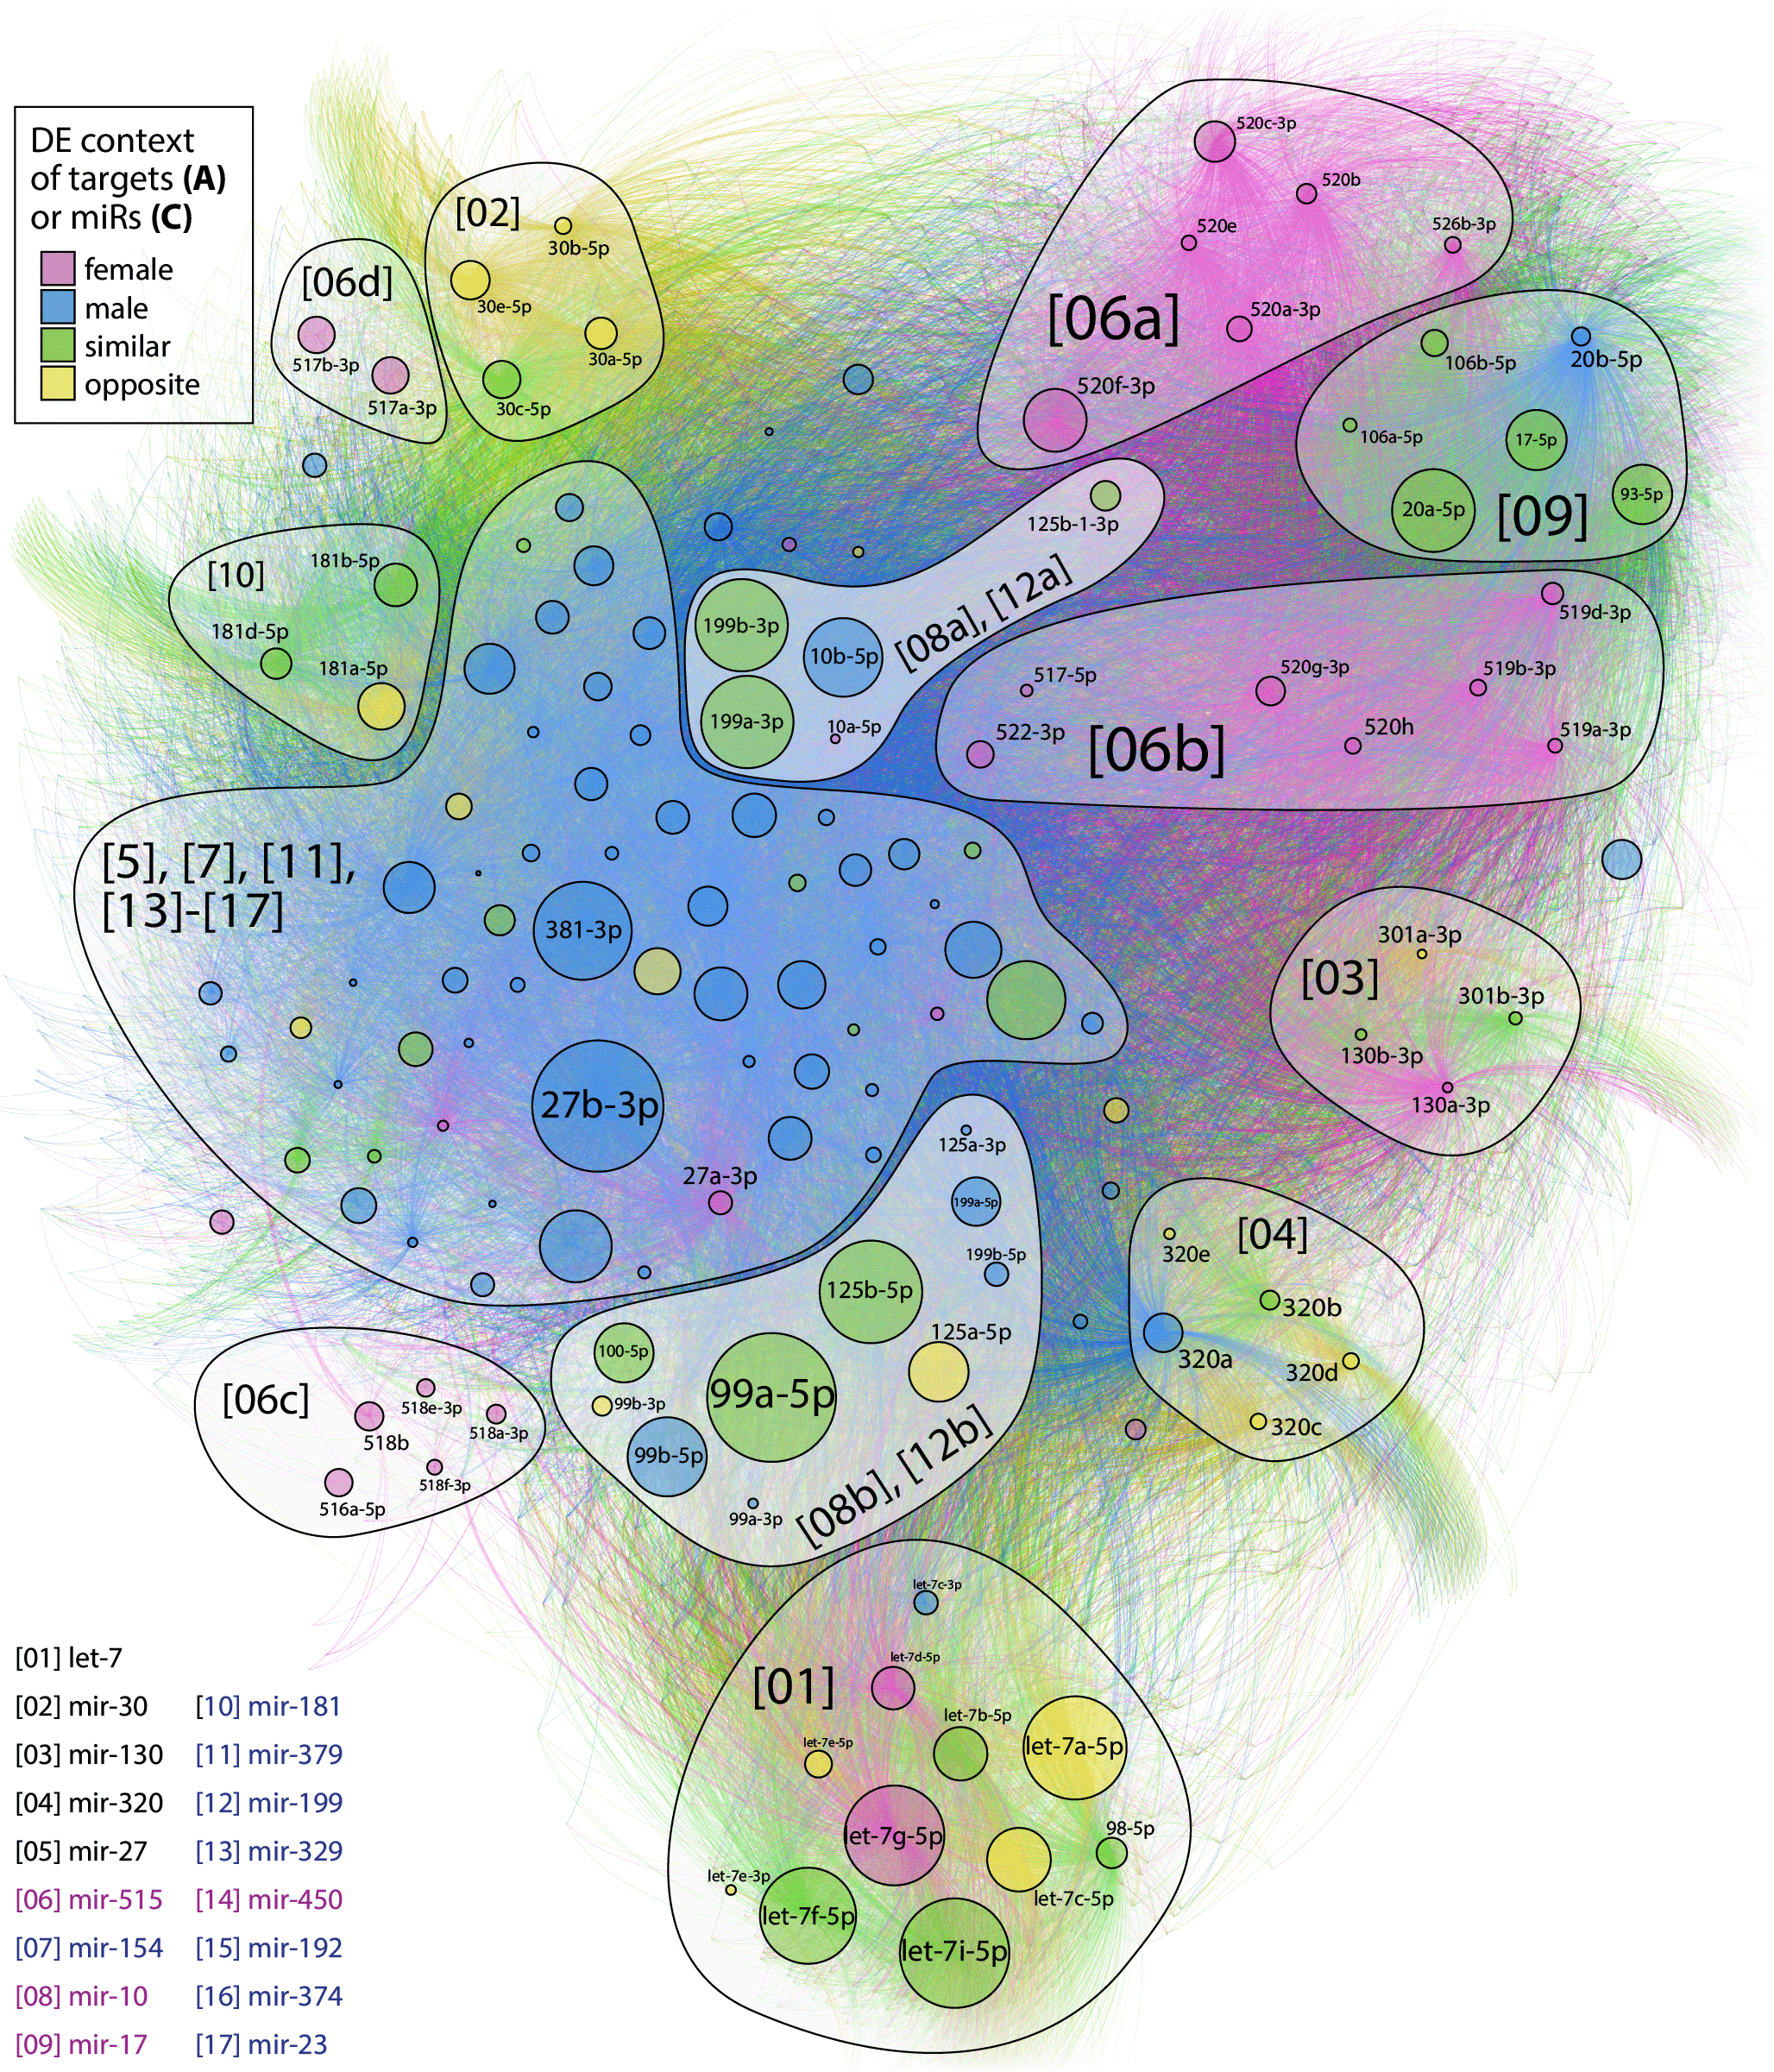
\includegraphics[width=\textwidth]{figures/bignet}
\caption[LA-N-2 / LA-N-5 Full Connectome.]{\textbf{Full Connectome of LA-N-2 and LA-N-5 Differentially Expressed miRNA Families.} The network of miRNA families and their \num{12495} targeted genes self-organises into a connectome map with \num{46937} unique edges. miRNA node size scaled by absolute count-change, nodes coloured by DE context. Numbers in brackets denote miRNA families, gene nodes have minimal size. By application of a force-directed layout, the miRNA families visibly self-segregate into clusters. The let-7 family, male-biased and female-biased clusters take up major parts of the network. Families mir-10 and mir-199, with neurokine association, form two mixed, sexually dimorphic clusters near the centre of the map (lighter shade).
\label{fig:bignet}}
\end{figure}

The resulting transcriptional connectome map illustrates the functional compartmentalisation of miRNA$\to$gene interactions. miRNAs of distinct families are frequently found in close proximity to one another, most often forming one or two clusters. In the case of two clusters forming, the clusters are usually representative of the two complementary strands of the pre-miRNA(s), since 3' and 5' variants of any pre-miRNA usually possess fundamentally different seed sequences, and thus, targets. The let-7 family is distinguished by its removal from the bulk of other interactions, possibly representing a particularly specialised set of functions, at least for the 5' variants of the bottom cluster\todo{evolutionary? discussion?}. Families with predominant differential expression in one of the two cell lines (sexes) inhabit different sides of the main graph and show little intermingling, pointing towards sexually dimorphic gene target distribution. The two neurokine-associated families, mir-10 and mir-199, are located near the centre of the graph, in two strand specific clusters (»[08a]\&[12a]« and »[08b]\&[12b]«.

To gather more detailed information than grouping of miRNAs with similar function, such as direct miRNA$\to$gene interaction, the size of the studied networks must be reduced. For each family affected by CNTF-differentiation, a single graph was created, laid out by application of ForceAtlas2, and analysed for critical nodes. The distinct families and their gene targets yield immensely diverse graph layouts, that here cannot be described in their entirety. However, the entire collection of graphs in interactive visual form is accessible at \url{https://slobentanzer.github.io/cholinergic-neurokine}. Due to an elevated interest, the cholinergic/neurokine miRNA interface and the families mir-10 and mir-199 will be described in more detail, and in conjunction with sex-specific perturbations in neurologic diseases.

%\section{The Cholinergic/Neurokine Interface}
%
%\begin{method}
%
%\subsection{Network Generation}
%To the set of cholinergic genes (see Box \ref{box:chol-genes}) were added: the genes for neurokines and their receptors, second messenger pathways (most importantly JAK/STAT), neurotrophin-related genes, and circadian genes.
%\todo{network of cholinergic/neurokine? mirs? both?}
%\todo{mir-125 ache culture test?}
%\todo{adjacency by targeted genes?}
%
%\end{method}


%!TEX root = ../dissertation.tex
\section{Application to Schizophrenia and Bipolar Disorder}
A comprehensive structural analysis of perturbations on a genome scale is hardly possible without heavy truncation of results or dimensionality reduction methods. Truncation is commonly performed by ranking perturbations by their p-values in ascending order and only regarding the highest ranked entries, which often amounts to less than ten individual transcripts. On the other hand, commonly used dimensionality reduction techniques include \ac{pca}, \ac{tsne}, and clustering/stratification approaches. While truncation enables human-readable presentation of results, in principle it does not lend itself to complex polygenic events such as neurologic disease. Common dimensionality reduction techniques are useful in providing structural overview of a high-dimensional dataset, but give little insight into causal relationships of single entities. We thus aimed to find an alternative approach to dimensionality reduction which conserves the internal relationships inherent to the data, and which profits from the network organisation of our input data.

For the application of \emph{miRNeo} data to real-world problems, suitable psychiatric and neurologic disease datasets were sought in the common repositories ArrayExpress, NCBI GEO, and Synapse. Among the datasets with agreeable quality, \ac{scz} and \ac{bd} were the only diseases with sample amounts that allowed a statistically valid analysis of sexual dimorphisms. While many neurologic disease studies are simply limited in their number of subjects, autism presented a different issue: the majority of donors were males (more than 90\%). Direct analysis of miRNA expression patterns was not possible, because very few studies study miRNAs directly, yet. Thus, studies on mRNA were substituted to infer on miRNA dynamics.

\begin{method}

\subsection{Analysed Datasets}
Twelve datasets including 1361 subjects were downloaded from their repositories (Table \ref{tab:datasets}). 
Data of DLPFC \ac{seq} of 579 SCZ patients and controls was obtained from the Common Mind Consortium (\url{http://www.synapse.org/CMC}). To address the diverse origins and technological aspects of data, care was taken to appropriately unify and normalise the data. The data preparation and meta analyses were performed essentially as described by Gandal and colleagues.\cite{Gandal2018} Samples of brain regions not consistent with the research question (e.g., cerebellum), or from patients with diseases other than SCZ or BD, were removed from datasets on a case-by-case basis. \ac{seq} datasets were used to individually confirm the perturbations found in the meta-analysis of microarray studies.

\begin{table}
\sffamily
\small
\centering
\begin{tabular}{c | c | c | c | c | c}
source & accession & publication & technology & subjects/samples & disease\\ \hline
\hline
NCBI GEO & GSE35978 & Chen \emph{et al.}\cite{Chen2013} & microarray & 150/312 & SCZ \& BD\\ \hline
NCBI GEO & GSE12649 & Iwamoto \emph{et al.}\cite{Iwamoto2005} & microarray & 102/102 & SCZ \& BD\\ \hline
NCBI GEO & GSE53987 & Lanz \emph{et al.}\cite{Lanz2015} & microarray & 76/205 & SCZ \& BD\\ \hline
NCBI GEO & GSE17612 & Maycox \emph{et al.}\cite{Maycox2009} & microarray & 51/51 & SCZ\\ \hline
NCBI GEO & GSE21138 & Narayan \emph{et al.}\cite{Narayan2008} & microarray & 30/59 & SCZ\\ \hline
NCBI GEO & GSE5392 & Ryan \emph{et al.}\cite{Ryan2006} & microarray & 82/82 & BD\\ \hline
NCBI GEO & GSE80655 & Ramaker \emph{et al.}\cite{Ramaker2017} & RNA-seq & 96/281 & SCZ \& BD\\ \hline
NCBI GEO & GSE106589 & Hoffman \emph{et al.}\cite{Hoffman2017} & RNA-seq & 94/94 & SCZ\\ \hline
NCBI GEO & GSE68559 & Webb \emph{et al.}\cite{Webb2015} & RNA-seq & 10/98 & NA\\ \hline
NCBI GEO & GSE96659 & Fontenot \emph{et al.}\cite{Fontenot2017} & RNA-seq & 5/209 & NA\\ \hline
NCBI GEO & GSE45642 & Li \emph{et al.}\cite{Li2013} & RNA-seq & 86/670 & NA\\ \hline
Synapse & CMC & Gulyás-Kovács \emph{et al.}\cite{Gulyas-Kovacs2018} & RNA-seq & 579/579 & SCZ \& BD\\ \hline
\end{tabular}
\caption{\textbf{Data Sources for Microarray and RNA-seq Analyses.}}
\label{tab:datasets}
\end{table}

\subsection{Microarray Quality Control and Data Preparation} \label{sec:cellculture:quality}
\subsubsection{Read-In and Normalisation}
Illumina datasets were read, log$_2$-transformed, and quantile-normalised using R/lumi.\cite{Du2008} Affymetrix datasets were read and RMA-normalised (log$_2$-transformed, background corrected, quantile-normalised) using R/affy.\cite{Gautier2004} Affymetrix data were additionally corrected for 3'/5' bias using the \emph{AffyRNAdeg()} function (not available for other chip manufacturers). All available biological (e.g., sex, age) and technical (e.g., batch, \ac{rin}, post-mortem interval) covariates were collected and used for the analysis. Individual correlations of case-control status $S$ with any covariate $C$ were assessed using a linear model (R/lm) with formula $C \smallsim S$; statistical significance was determined via ANOVA (R/anova). If necessary, case-control samples were balanced to eliminate significant covariate correlations with case-control status (all p > 0.05).

\subsubsection{Outliers}
Outlier removal was performed using the method proposed by Oldham, Langfelder \& Horvath.\cite{Oldham2012} Briefly, the (dis\-/)similarity matrix of samples is transformed into a signed, weighted correlation network. Network adjacency ($a$) of samples (nodes) $S_i$ and $S_j$ is defined as: $$a_{ij} = \left(\frac{cor(S_i, S_j)+1}{2}\right)^2$$

As such, the connectivity between samples can be measured by the standardised connectivity (\emph{Z.K}), which describes the strength of correlation between any given node and all other nodes in the network. As proposed by Oldham \emph{et al.}, outliers were removed if their Z-score was below the threshold of \emph{Z.K} = -2.

\subsubsection{Annotation}
To enable comparison between datasets of diverse technical origin, probes were annotated using ENSEMBL gene identifiers using R/biomaRt.\cite{Durinck2009} To maintain comparability with the analysis by Gandal \emph{et al},\cite{Gandal2018} the same version of ENSEMBL DB (v75, Feb 2014) was used. Probes were collapsed onto single genes using the \emph{collapseRows()} function of R/WGCNA,\cite{Langfelder2008} using the maximum mean signal across all probes per gene. Of note, information loss occured by multiple collapsing of probes and integration of datasets, which can only be performed using the genes common to all datasets (i.e., represented by microarray probes). The final gene set encompassed 12\,391 individual genes, with several notable cholinergic/neurokine exceptions (CHRNA7, CHRM1, LHX8, CHKB, PRIMA1, CNTF). Missing genes result from annotation deficits between different probe sets, cannot be comprehensively manually controlled on a genome scale, and cannot be re-introduced at this stage. 

\subsection{Differential Expression Meta-Analysis}
The individual experimental datasets were each corrected for covariate influences by multiple regression based on all available biological and technical covariates. Briefly, the linear regression model was solved using matrix algebra operations. In matrix form, a linear regression model of observations $Y$ (i.e., gene expression levels), independent variables $X$ (i.e., covariates), coefficients $\beta$, and error terms $\epsilon$ can be described as: $$Y = X\beta + \epsilon$$ As a consequence, the residual sums of squares can be expressed as the cross product: $$RSS = (Y - X\beta)^T(Y - X\beta)$$ Then, the coefficients $\hat{\beta}$ can be estimated by solving the derivative: $$\hat{\beta} = (X^TX)^{-1} X^TY$$ Coefficients were estimated for all relevant technical and biological covariates (e.g. post-mortem interval, RIN, sex, age) and used to regress covariate influence on gene expression levels: $$Y_{new} = Y - (X\hat{\beta})^T$$

After covariate regression, differential expression was calculated across all datasets for each disease group using a linear mixed model with a fixed effect for each study and case-control status (»group«), and a random effect for each individual subject. Computation was performed in R, using R/nlme,\cite{Pinheiro2019} with parameters $$fixed = \smallsim group + study\textrm{\sffamily\,\,\,and\,\,\,}random = \smallsim 1|subject$$

This yielded an array of log-fold changes between cases and controls for each gene and disease. To determine statistical significance, 10\,000 permutations of the mixed-model regression were performed for each use case, randomly assigning case-control status. The resulting null distributions were used to determine \ac{fdr}, with threshold for significance at 0.05. 

\subsubsection{Sex-Specific Meta-Analysis}
Samples of all datasets were split between males and females (cases as well as controls), and individually subjected to the same procedure as the sex-independent data: covariate regression, differential expression via a linear mixed model, and estimation of statistical significance via permutation testing.

\subsubsection{Transcriptome Correlation}
Correlation of disease transcriptomes was performed by using Spearman's rank correlation coefficient. Spearman's $\rho$ was determined between SCZ and BD sex-independently as well as separately in males and females.

\subsubsection{Most Diverging Genes}
Genes were ranked by their divergence between any two compared datasets, sex-independent data of SCZ and BD, and any meaningful combination of sex-dependent data in SCZ, BD, males, and females. The divergence $\updelta$ of any gene $G$ between datasets $i$ and $j$ was defined as (\emph{logFC}: log-fold change): $$\updelta = logFC(G)_i - logFC(G)_j$$

Where positive values of $\updelta$ indicate a positive bias of $G$ towards dataset $i$.

\end{method}

\subsection{Sexual Dimorphism in Schizophrenia and Bipolar Disorder}
Sex-independent correlation replicated the finding of Gandal \emph{et al},\cite{Gandal2018} with Spearman's $\rho = 0.7100$ \mbox{(p < 0.001)}. However, diverging from the established annotation of ENSEMBL v75 to later versions of the database significantly altered the correlation coefficient, leading to lower correlation in all tested cases. Comparing the sex-independent data with only male or female subjects, those also show lower general correlation between SCZ and BD: in females, correlation was $\rho = 0.6150$ (p < 0.001), in males, $\rho = 0.5783$ (p < 0.001). While it is possible that these variations are caused by structural properties of the data unrelated to sexual dimorphism, such as the loss of power due to the reduction in size, the consistently lower correlation in sex-specific subsets also may indicate an averaging effect between male and female patients, leading to a higher correlation in spite of significant sexual dimorphism.

 To address the potential differences between male and female brain transcriptomes, which may reflect the observed clinical dimorphism, we subjected the 100 most-diverging genes between any two datasets to \ac{go} enrichment analysis (Fig.\,\ref{fig:scz-bd-go}, from Lobentanzer \emph{et al.}\cite{Lobentanzer2019a}) in hopes of identifying the most discriminating molecular pathways between SCZ and BD, and afflicted males and females. Sex-independently, the most-diverging pathways between SCZ and BD principally involved mechanisms of inflammation and immunity (e.g., ‘‘acute inflammatory response,’’ p = 0.003; ‘‘cellular response to cytokine stimulus,’’ p = 0.01).

\subsubsection{Differences in Sexual Dimorphism Between SCZ and BD}
Computation of diverging pathways between males and females in each disease indicated a larger divergence between sexes in SCZ than in BD. SCZ-biased genes of males and females showed no overlapping GO terms (Fig.\,\ref{fig:scz-bd-go}\,A), but BD-biased genes of males and females showed large GO term overlap, particularly in inflammatory components (Fig.\,\ref{fig:scz-bd-go}\,B). Notably, specific components of neurokine signalling were elevated in both males (IL-6, p= 0.007) and females (JAK/STAT, p = 0.01) with BD.

\subsubsection{Overlap of Male-Biased Genes Between SCZ and BD}
Shared transcriptional properties of SCZ and BD were identifiable only in male diverging genes. While female-biased SCZ genes showed no implications in CNS processes, male-biased SCZ and BD genes overlapped in functions concerning inflammation and immunity (Fig.\,\ref{fig:scz-bd-go}\,C). Female-biased BD genes were associated with CNS function and development (Fig.\,\ref{fig:scz-bd-go}\,D).

\begin{figure}[ht]
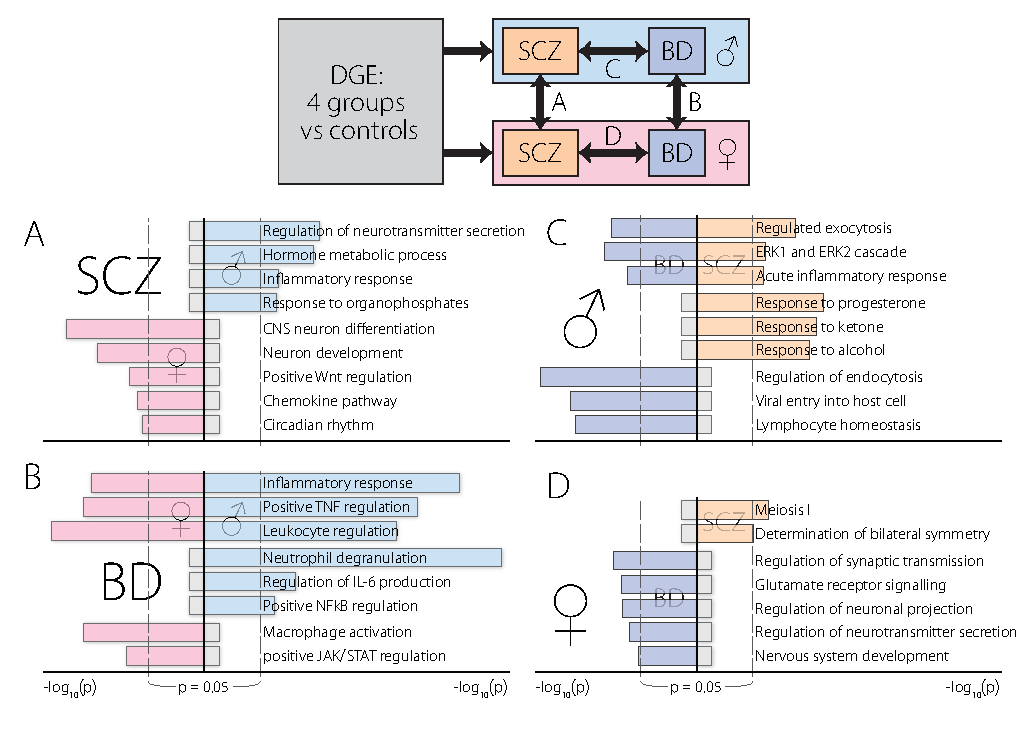
\includegraphics[width=\textwidth]{figures/scz-bd-go}
\caption[GO Enrichment of Diverging Genes.]{\textbf{GO Enrichment of Diverging Genes.} Results of differential gene expression were dually compared: SCZ versus BD and male versus female (indicated by colours). GO enrichment of the top 100 distinguishing genes in one dimension was compared with the other for each pair of combinations. \textbf{A)} SCZ-biased genes diverge between males and females. \textbf{B)} BD-biased genes share immunological ontology in both males and females. \textbf{C)} Male-biased genes share immunological ontology in BD and SCZ. \textbf{D)} Female-biased genes diverge between SCZ and BD.
\label{fig:scz-bd-go}}
\end{figure}

\subsubsection{Specificity of Ontological Terms}
When comparing different areas of biological function, such as neurotransmission, immunity, and inflammation, the different areas notably diverged in the specificity of identified terms. Considering the functionality of the applied method (\emph{topGO}, see Section \ref{sec:cellculture:topgo}) to find the most specific node in any branch of the \ac{dag} tree while disregarding its (less specific) parent nodes, this may indicate a difference in the gravity of perturbation in the different systems. For instance, the GO terms indicating neurotransmission as affected system were much less specific than those indicating immunity-related processes. While significant neurotransmission-related terms failed to implicate specific neuron types or neurotransmitters (e.g., GO:0021953, »CNS neuron differentiation«; GO:0046928, »Regulation of neurotransmitter secretion«), immunity-related terms were very specific towards regulatory subsystems, and regularly implicated neurokine mechanisms (e.g., GO:0032675, »Regulation of interleukin-6 production«; GO:0046427, »Positive regulation of JAK/STAT cascade«).

\subsection{Combination of Disease Data and Cell Culture}
To implement the proposed complexity reduction technique, we applied a reductionist approach to the comprehensive network generated from perturbed miRNA families and their targeted genes (Fig.\,\ref{fig:bignet}), based on the unbiased analysis of sexual dimorphism in SCZ and BD, which implicated processes of neuronal, immunological, and circadian origin (Figure \ref{fig:scz-bd-go}). To merge these results with the implications of cholinergic cell culture, we added genes implicated in neurokine signaling and circadian rhythm to the list of cholinergic genes (see Box \ref{box:chol-genes}). Returning to the collection of web-available patient data, we subjected this limited set of 76 genes and their 18 neuronal TFs to differential expression analysis.

The comprehensive network was then filtered by multiple consecutive steps. (I) Permutation analysis of comprehensive miRNA targeting data specific for genes expressed in cholinergic neurons (Fig.\,\ref{fig:singlecell}) yielded a list of miRNA candidates that shows overlap with (II) miRNAs DE in our two models of neurokine-induced cholinergic differentiation (Fig.\,\ref{fig:cc-cor-de-perm}\,A). (III) We included only families of miRNAs we found to be enriched in differential expression (Fig.\,\ref{fig:mir-de-fam-go}). Sixty-nine miRNAs from 12 families passed this filtering process and were consecutively assembled in a force-directed network with the 94 genes of the previously compiled list. As a »spike-in«, we added miR-132-3p (DE in LA-N-5 cells), a miRNA which controls cholinergic processes\cite{Shaltiel2013, Hanin2018} and is known for its function in neurons\cite{Mellios2011} and immunity\cite{Shaked2009} and its perturbation in disease.\cite{Pichler2017} The resulting network (Fig.\,\ref{fig:smallnet}\,A, from Lobentanzer \emph{et al.}\cite{Lobentanzer2019a}) shows high structural homology to the comprehensive network shown in Figure \ref{fig:bignet}. The miRNA families in this reduced network show spatial organisation similar to the comprehensive network. 

\begin{figure}[ht]
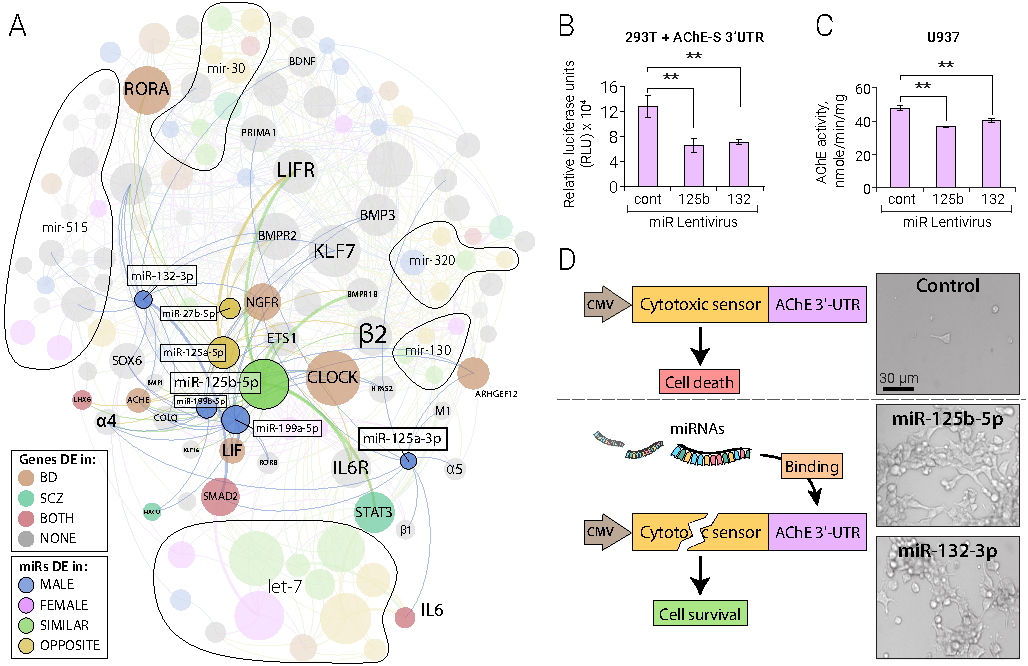
\includegraphics[width=\textwidth]{figures/smallnet}
\caption[The cholinergic/neurokine interface.]{\textbf{The cholinergic/neurokine interface.} \textbf{A)} The miRNA families mir-10 and mir-199 pose a sexually dimorphic interface of cholinergic, neurokine, and circadian regulation by targeting nicotinic/ muscarinic (e.g., a4b2 and M1) and neurokine receptors, transcriptional regulators of cholinergic differentiation (LHX and STAT) and circadian rhythm (CLOCK and RORA), the AChE and the AChE linker proteins PRIMA1/COLQ, and high-affinity choline uptake (HACU). Members of mir-10/199 families, spike-in miR-132-3p, and their targeted genes are shown in colour, and other miRNA families that passed the multiple filtering are indicated as areas. miRNA node size corresponds to count-change and gene node size to connectivity; colour and thicker edges indicate the DE context and experimentally validated connections. \textbf{B–D} Validation experiments of AChE targeting by miR-125b-5p, with miR-132-3p as a positive control. \textbf{B)} Lentiviral expression of miR-132 and miR-125b suppresses luciferase fused to the 3' UTR of AChE in HEK293T cells. Error bars indicate SE. \textbf{C)} Lentiviral expression of miR-132 and miR-125b suppresses the endogenous AChE hydrolytic activity of U937 cells with similar efficacy. Error bars indicate SE. \textbf{D)} Life/death assay of stably transfected HEK293T cells carrying the AChE 3' UTR fused to a cytotoxic sensor and co-transfected with miR-125b-5p, miR-132-3p, or control plasmids. Cells survive in case of binding of miR-132-3p and miR-125-5p to the 3' UTR.
\label{fig:smallnet}}
\end{figure}

In agreement with their localisation in the comprehensive network, miRNA families mir-10 and mir-199 inhabit a central role in the resulting interactome. Most-targeted genes in this network (as indicated by their size) are the circadian regulators CLOCK and \acs{rora}. While CLOCK is located centrally, next to mir-10/199 miRNAs, RORA shows closeness to the mir-30/515 families. Generally, genes with larger cellular influence, such as transcription factors (STAT3, CLOCK) or \ac{tgf}-$\upbeta$ ligands (BMP family genes) are frequently targeted by miRNAs, while more specific transcripts, such as the cholinergic receptor genes or neurokines, are targeted more selectively. \todo{more details?}

More so than the spiked-in miR-132-3p, mir-10/199 miRNAs target cholinergic genes, for instance, the neuronal nicotinic $\upalpha4\upbeta2$ and muscarinic M1 receptors (mir-125) and HACU (miR-199). In addition, they target neurokine genes, such as the transmembrane neurokine receptor LIFR or STAT3, and circadian regulators (e.g., CLOCK and RORA). The two families react highly sexually dimorphic to CNTF-mediated differentiation; some are detected as \ac{de} only in one cell line, others exhibit inverted changes between cell lines. The 3p-variant of miR-125a distinguishes itself from the bulk of mir-10/199 miRNAs by exclusively targeting M1, $\upalpha5$ and $\upbeta1$ receptors, and IL-6, and thus is slightly removed from the centre of the network. \todo{Describe other members?}

The miRNA with most targets in this reduced interactome is miR-125b-5p, also displaying most experimentally validated interactions with neurokine genes (miRTarBase accessions: IL-6, MIRT\-022105; IL-6R, MIRT006844; JAK2, MIRT734987; LIF, MIRT001037; LIFR, MIRT732494; \linebreak STAT3, MIRT005006). miR-125b-5p also is the most perturbed miRNA (in this interactome) upon CNTF-mediated differentiation (highest count-change), and the only member of mir-10/mir-199 to be changed in similar direction in both cell lines (up-regulated). miR-125b-5p also targets multiple other inflammation-related genes (e.g., \ac{tnf}, MIRT733472; IRF4, MIRT004534) and 5-lipoxygenase, which can influence inflammatory processes via production of eicosanoids.\cite{Busch2015} miR-125b-5b has been directly associated with cytokine-mediated inflammation, as its over-expression increased the expression of \ac{tnf}-$\upalpha$, IL-1$\upbeta$, and IL-6, and markedly decreased I$\upkappa$B-$\upalpha$.\cite{Zhang2017}

A notable intersection of spike-in miR-132-3p and miR-125b-5p is the \ac{ache}, an interaction which had not been validated for miR-125b-5p, but is known for miR-132-3p.\cite{Shaked2009, Shaltiel2013} Using miR-132-3p as a positive control, we performed ACHE-mRNA binding assays in validation of the predicted targeting by miR-125b-5p.

\begin{method}

\subsection{miR-125b-5p Acetylcholinesterase Targeting Assays}
We performed three independent cell culture assays to confirm \emph{ACHE} mRNA targeting by hsa-miR-125b-5p: luciferase suppression, AChE protein activity, and a cell death assay with a cytotoxic sensor. The 3' UTR of human \emph{ACHE} mRNA\cite{Soreq1990} was cloned into the microRNA Target Selection System plasmid (System Biosciences, CA, USA) multiple cloning site, using EcoRI and NotI restriction enzymes (New England Biolabs). All plasmids were verified by DNA sequencing. For luciferase assays, HEK293T cells were transfected with miRNA Target Selection-AChE-3' UTR, and selected in the presence of Puromycin for 3 weeks. Stably transfected HEK293T (293T-AChE 3' UTR) cells were grown on 12-well plates and infected with lentiviruses expressing miR-125b-5p, miR-132-3p or a negative control sequence. After 48 hours incubation, cells were analysed using the Dual Luciferase Assay kit (Promega, WI USA) and Luciferase activity was measured using an Envision luminescent plate reader (Perkin-Elmer, Waltham, MA), essentially as previously described by Hanin \emph{et al.}\cite{Hanin2014} For each reporter construct, renilla luciferase activity was normalized according to that of the firefly. Normalised activity after infection with miR-132-3p or miR-125b-5p was expressed as relative to that obtained after infection with the same plasmid with miRNA negative control. To show effects of changes in this miRNA’s levels on real-life protein activities, we performed an AChE hydrolytic activity assay following infection of human monocyte-like U937 cells with hsa-miR-125b-5p, miR-132-3p or a negative control lentiviral vector. AChE hydrolytic activity levels were assessed by kinetic measurements of the hydrolysis rates of \SI{1}{\milli\Molar} acetylthiocholine (ATCh, Sigma) at room temperature, following 20 min incubation with and without \SI{50}{\micro\Molar} tetraisopropyl pyrophosphoramide (iso-OMPA, Sigma), a specific inhibitor of butyrylcholinesterase, to selectively assay for AChE-specific or total cholinesterase activity. For the life/death assay, stably transfected HEK293T cells were infected with lentiviruses expressing miR-125b-5p, miR-132-3p or a negative control sequence. 72 hours post-infection, a cytotoxic reporter fused to AChE 3' -UTR was added to the media and cells were kept for an additional 5 days to assess their viability. For all cell culture assays, statistical significance was determined using ANOVA with correction for multiple testing. Each sample was assayed in at least 3 biological replicates, and in all cases, hsa-miR- 132-3p served as a positive control.

\end{method}

\subsection{hsa-miR-125b-5p Targets Acetylcholinesterase}
In all tested conditions, miR-125b-5p suppressed \emph{ACHE} mRNA with equal potency as the positive control miR-132-3p (Fig.\,\ref{fig:smallnet}\,B-D). Towards mRNA expression (luciferase) and functionality (cytotoxic sensor) as well as on protein level (AChE activity), miR-125b-5p demonstrated its interaction with ACHE mRNA 3' UTR. Luciferase units after miR-125b-5p transfection were approximately halved, indicating significant transcript degradation of the \emph{ACHE} 3'UTR.

\subsection{Cholinergic/Neurokine Mechanisms in Web-Available\\ RNA Sequencing Experiments}
To include recent developments in methodology, we analysed several recent \ac{seq} studies addressing related questions. In a study of post-mortem brain transcriptome profiling of psychiatric disorders,\cite{Ramaker2017} we found a down-regulation of IL-6, LIF, and several cholinergic receptors (M2, M4, $\upalpha$4, $\upbeta$2, $\upalpha$7), with sex-specific differences (males had significantly higher levels of neurokines than females). These changes were visible only in SCZ patients, not in BD or major depressive disorder. In a study of \acp{ipsc} of SCZ patients and controls that were induced to show a neuronal phenotype,\cite{Hoffman2017} we found an up-regulation of \emph{CHAT} in SCZ-derived iPSCs, and a down-regulation of IL6R and the nicotinic $\upalpha$6 subunit. In this study, SCZ males showed a higher expression of the \emph{SLC18A3} and lower expression of nicotinic subunits $\upalpha$ 2, 7, and 9, and $\upbeta$3. In a study of differentiated human neuronal progenitor cells,\cite{Fontenot2017} a knockdown of the circadian transcriptional controller CLOCK resulted in up-regulation of LIF and simultaneous down-regulation of neurokine transmembrane receptors LIFR and IL6ST, accompanied by slight bi-directional changes in several cholinergic receptors.


%\begin{table}
%\centering
%\begin{tabular}{c | c | c | c}
%family name & LA-N-2 p-value & LA-N-5 p-value & implicated in disease\\ \hline
%\hline
%let-7 & 1.2E-3 & 1.5E-7 & disease\\ \hline
%mir & pval & pval & disease\\ \hline
%\end{tabular}
%\caption{Enriched miRNA families in CNTF-induced differential expression in LA-N-2 and LA-N-5.}
%\label{tab:mir-de-fam}
%\end{table}
